% Options for packages loaded elsewhere
\PassOptionsToPackage{unicode}{hyperref}
\PassOptionsToPackage{hyphens}{url}
%
\documentclass[
  spanish,
]{book}
\usepackage{amsmath,amssymb}
\usepackage{lmodern}
\usepackage{iftex}
\ifPDFTeX
  \usepackage[T1]{fontenc}
  \usepackage[utf8]{inputenc}
  \usepackage{textcomp} % provide euro and other symbols
\else % if luatex or xetex
  \usepackage{unicode-math}
  \defaultfontfeatures{Scale=MatchLowercase}
  \defaultfontfeatures[\rmfamily]{Ligatures=TeX,Scale=1}
\fi
% Use upquote if available, for straight quotes in verbatim environments
\IfFileExists{upquote.sty}{\usepackage{upquote}}{}
\IfFileExists{microtype.sty}{% use microtype if available
  \usepackage[]{microtype}
  \UseMicrotypeSet[protrusion]{basicmath} % disable protrusion for tt fonts
}{}
\makeatletter
\@ifundefined{KOMAClassName}{% if non-KOMA class
  \IfFileExists{parskip.sty}{%
    \usepackage{parskip}
  }{% else
    \setlength{\parindent}{0pt}
    \setlength{\parskip}{6pt plus 2pt minus 1pt}}
}{% if KOMA class
  \KOMAoptions{parskip=half}}
\makeatother
\usepackage{xcolor}
\IfFileExists{xurl.sty}{\usepackage{xurl}}{} % add URL line breaks if available
\IfFileExists{bookmark.sty}{\usepackage{bookmark}}{\usepackage{hyperref}}
\hypersetup{
  pdftitle={Series de Tiempo},
  pdfauthor={Omar Rodríguez Torres (omarr667@ciencias.unam.mx)},
  pdflang={es},
  hidelinks,
  pdfcreator={LaTeX via pandoc}}
\urlstyle{same} % disable monospaced font for URLs
\usepackage{color}
\usepackage{fancyvrb}
\newcommand{\VerbBar}{|}
\newcommand{\VERB}{\Verb[commandchars=\\\{\}]}
\DefineVerbatimEnvironment{Highlighting}{Verbatim}{commandchars=\\\{\}}
% Add ',fontsize=\small' for more characters per line
\usepackage{framed}
\definecolor{shadecolor}{RGB}{248,248,248}
\newenvironment{Shaded}{\begin{snugshade}}{\end{snugshade}}
\newcommand{\AlertTok}[1]{\textcolor[rgb]{0.94,0.16,0.16}{#1}}
\newcommand{\AnnotationTok}[1]{\textcolor[rgb]{0.56,0.35,0.01}{\textbf{\textit{#1}}}}
\newcommand{\AttributeTok}[1]{\textcolor[rgb]{0.77,0.63,0.00}{#1}}
\newcommand{\BaseNTok}[1]{\textcolor[rgb]{0.00,0.00,0.81}{#1}}
\newcommand{\BuiltInTok}[1]{#1}
\newcommand{\CharTok}[1]{\textcolor[rgb]{0.31,0.60,0.02}{#1}}
\newcommand{\CommentTok}[1]{\textcolor[rgb]{0.56,0.35,0.01}{\textit{#1}}}
\newcommand{\CommentVarTok}[1]{\textcolor[rgb]{0.56,0.35,0.01}{\textbf{\textit{#1}}}}
\newcommand{\ConstantTok}[1]{\textcolor[rgb]{0.00,0.00,0.00}{#1}}
\newcommand{\ControlFlowTok}[1]{\textcolor[rgb]{0.13,0.29,0.53}{\textbf{#1}}}
\newcommand{\DataTypeTok}[1]{\textcolor[rgb]{0.13,0.29,0.53}{#1}}
\newcommand{\DecValTok}[1]{\textcolor[rgb]{0.00,0.00,0.81}{#1}}
\newcommand{\DocumentationTok}[1]{\textcolor[rgb]{0.56,0.35,0.01}{\textbf{\textit{#1}}}}
\newcommand{\ErrorTok}[1]{\textcolor[rgb]{0.64,0.00,0.00}{\textbf{#1}}}
\newcommand{\ExtensionTok}[1]{#1}
\newcommand{\FloatTok}[1]{\textcolor[rgb]{0.00,0.00,0.81}{#1}}
\newcommand{\FunctionTok}[1]{\textcolor[rgb]{0.00,0.00,0.00}{#1}}
\newcommand{\ImportTok}[1]{#1}
\newcommand{\InformationTok}[1]{\textcolor[rgb]{0.56,0.35,0.01}{\textbf{\textit{#1}}}}
\newcommand{\KeywordTok}[1]{\textcolor[rgb]{0.13,0.29,0.53}{\textbf{#1}}}
\newcommand{\NormalTok}[1]{#1}
\newcommand{\OperatorTok}[1]{\textcolor[rgb]{0.81,0.36,0.00}{\textbf{#1}}}
\newcommand{\OtherTok}[1]{\textcolor[rgb]{0.56,0.35,0.01}{#1}}
\newcommand{\PreprocessorTok}[1]{\textcolor[rgb]{0.56,0.35,0.01}{\textit{#1}}}
\newcommand{\RegionMarkerTok}[1]{#1}
\newcommand{\SpecialCharTok}[1]{\textcolor[rgb]{0.00,0.00,0.00}{#1}}
\newcommand{\SpecialStringTok}[1]{\textcolor[rgb]{0.31,0.60,0.02}{#1}}
\newcommand{\StringTok}[1]{\textcolor[rgb]{0.31,0.60,0.02}{#1}}
\newcommand{\VariableTok}[1]{\textcolor[rgb]{0.00,0.00,0.00}{#1}}
\newcommand{\VerbatimStringTok}[1]{\textcolor[rgb]{0.31,0.60,0.02}{#1}}
\newcommand{\WarningTok}[1]{\textcolor[rgb]{0.56,0.35,0.01}{\textbf{\textit{#1}}}}
\usepackage{longtable,booktabs,array}
\usepackage{calc} % for calculating minipage widths
% Correct order of tables after \paragraph or \subparagraph
\usepackage{etoolbox}
\makeatletter
\patchcmd\longtable{\par}{\if@noskipsec\mbox{}\fi\par}{}{}
\makeatother
% Allow footnotes in longtable head/foot
\IfFileExists{footnotehyper.sty}{\usepackage{footnotehyper}}{\usepackage{footnote}}
\makesavenoteenv{longtable}
\usepackage{graphicx}
\makeatletter
\def\maxwidth{\ifdim\Gin@nat@width>\linewidth\linewidth\else\Gin@nat@width\fi}
\def\maxheight{\ifdim\Gin@nat@height>\textheight\textheight\else\Gin@nat@height\fi}
\makeatother
% Scale images if necessary, so that they will not overflow the page
% margins by default, and it is still possible to overwrite the defaults
% using explicit options in \includegraphics[width, height, ...]{}
\setkeys{Gin}{width=\maxwidth,height=\maxheight,keepaspectratio}
% Set default figure placement to htbp
\makeatletter
\def\fps@figure{htbp}
\makeatother
\setlength{\emergencystretch}{3em} % prevent overfull lines
\providecommand{\tightlist}{%
  \setlength{\itemsep}{0pt}\setlength{\parskip}{0pt}}
\setcounter{secnumdepth}{5}
\usepackage{booktabs}
\usepackage{xcolor} 
\definecolor{gray97}{gray}{.97}
\definecolor{gray97}{gray}{.97}
\definecolor{airforceblue}{rgb}{0.36, 0.54, 0.66}
\definecolor{Mahogany}{rgb}{0.75, 0.25, 0.0}
\definecolor{Olive}{rgb}{0.5, 0.5, 0.0}
\definecolor{colortitulo}{RGB}{219,68,14} % 
\definecolor{colordominante}{RGB}{243,102,25}
\definecolor{colordominanteF}{RGB}{219,68,14}
\definecolor{colordominanteD}{RGB}{137,46,55}
\definecolor{mostaza}{RGB}{231,196,25}
\definecolor{amarilloM}{RGB}{248,199,90}
\definecolor{amarilloD}{RGB}{251,237,121}
\definecolor{grisamarillo}{RGB}{248,248,245} 
\definecolor{azulF}{rgb}{.0,.0,.3}
\definecolor{grisD}{rgb}{.3,.3,.3}
\definecolor{grisF}{rgb}{.82,.82,.82}
\definecolor{miverde}{RGB}{44,162,67}
\newcommand{\verde}{\color{miverde}}

\usepackage{listings}
% Puede usar lstlisting|texto| para código en el texto
\lstset{ 
	language=R,                     % the language of the code
	basicstyle=\footnotesize\ttfamily, % the size of the fonts that are used for the code
	%numbers=left,                   % where to put the line-numbers
	%numberstyle=\tiny\color{Blue},  % the style that is used for the line-numbers
	%stepnumber=1,                   % the step between two line-numbers. If it is 1, each line
	% will be numbered
	%numbersep=5pt,                  % how far the line-numbers are from the code
	frame=single,
	framextopmargin=3pt,
	framexbottommargin=3pt,
	framexleftmargin=0.4cm,
	backgroundcolor=\color{gray97},
	showspaces=false,               % show spaces adding particular underscores
	showstringspaces=false,         % underline spaces within strings
	showtabs=false,                 % show tabs within strings adding particular underscores
	frame=single,                   % adds a frame around the code
	rulecolor=\color{black},        % if not set, the frame-color may be changed on line-breaks within not-black text (e.g. commens (green here))
	tabsize=2,                      % sets default tabsize to 2 spaces
	captionpos=b,                   % sets the caption-position to bottom
	breaklines=true,                % sets automatic line breaking
	breakatwhitespace=false,        % sets if automatic breaks should only happen at whitespace
	keywordstyle=\color{Mahogany},      % keyword style
	commentstyle=\color{airforceblue},   % comment style
	stringstyle=\color{Olive}      % string literal style
} 


%\usepackage[width=17cm,height=23cm]{geometry}
%\geometry{bindingoffset=1.2cm}
\textheight=22cm
\textwidth=15.5cm
\topmargin=-1cm
\oddsidemargin = -0cm %margen izquierdo, página impar
\evensidemargin = -0cm %margen izquierdo, página par

\newcommand{\helv}{\fontfamily{phv}\fontsize{9}{11}\selectfont}


\usepackage{fancyhdr}
\pagestyle{fancy}

\renewcommand{\chaptermark}[1]{\markboth{#1}{}}
\renewcommand{\sectionmark}[1]{\markright{\thesection\ #1}}
\fancyhf{} % borra cabecera y pie actuales
\fancyhead[LE,RO]{\helv\thepage} %Left Even page - Right Odd page
\fancyhead[LO]{\helv\rightmark}
\fancyhead[RE]{\helv\leftmark}
%\renewcommand{\headrulewidth}{0pt} % Sin raya. Con raya?: cambiar {0} por {0.5pt}
%\renewcommand{\footrulewidth}{0pt}
\renewcommand{\headrulewidth}{0.5pt} % grosor 0.5pt
\addtolength{\headheight}{0.5pt} % espacio para la raya
\fancyheadoffset{0 cm} %Controla el tamaño de la línea



\usepackage{mdframed}

\usepackage{amsthm}
\newtheorem{theorem}{Teorema}[chapter]
\newtheorem{lemma}{Lema}[chapter]
\newtheorem{corollary}{Corolario}[chapter]
\newtheorem{proposition}{Proposición}[chapter]
\newtheorem{conjecture}{Conjecture}[chapter]

\newtheorem{del}{Definición}[chapter]
\newenvironment{definition}
{\begin{mdframed}[backgroundcolor=grisF, rightline=false,leftline=false,topline=false, bottomline=false]\begin{del}}
		{\end{del}\end{mdframed}}

\newtheorem{example}{Ejemplo}[chapter]
\newtheorem{exercise}{Ejercicio}[chapter]
\newtheorem{hypothesis}{Hypothesis}[chapter]
\theoremstyle{remark}
\newtheorem*{remark}{Nota: }
\newtheorem*{solution}{Solución}

\parskip=0.4cm
\parindent=3mm
\usepackage{booktabs}
\usepackage{longtable}
\usepackage{array}
\usepackage{multirow}
\usepackage{wrapfig}
\usepackage{float}
\usepackage{colortbl}
\usepackage{pdflscape}
\usepackage{tabu}
\usepackage{threeparttable}
\usepackage{threeparttablex}
\usepackage[normalem]{ulem}
\usepackage{makecell}
\usepackage{xcolor}
\ifXeTeX
  % Load polyglossia as late as possible: uses bidi with RTL langages (e.g. Hebrew, Arabic)
  \usepackage{polyglossia}
  \setmainlanguage[]{spanish}
\else
  \usepackage[main=spanish]{babel}
% get rid of language-specific shorthands (see #6817):
\let\LanguageShortHands\languageshorthands
\def\languageshorthands#1{}
\fi
\ifLuaTeX
  \usepackage{selnolig}  % disable illegal ligatures
\fi
\usepackage[]{natbib}
\bibliographystyle{apalike}

\title{Series de Tiempo}
\author{Omar Rodríguez Torres (\href{mailto:omarr667@ciencias.unam.mx}{\nolinkurl{omarr667@ciencias.unam.mx}})}
\date{2021-07-14}

\begin{document}
\maketitle

{
\setcounter{tocdepth}{1}
\tableofcontents
}
\hypertarget{pruxf3logo}{%
\chapter*{Prólogo}\label{pruxf3logo}}
\addcontentsline{toc}{chapter}{Prólogo}

Estas notas corresponden al curso de Modelos de Supervivencia y de Series de Tiempo contemplados en el \href{http://www.fciencias.unam.mx/licenciatura/asignaturas/2017/1739}{plan de estudio} en la Facultad de Ciencias de la Universidad Nacional Autónoma de México para las licenciaturas de actuaría, matemáticas y matemáticas aplicadas.

El siguiente texto esta enfocado para los interesados que desean abordar el tema de series de tiempo, aunque su lectura puede ser relevante para cualquier interesado se desea que el lector tenga conocimientos solidos en probabilidad y en temas de estadística inferencial, así por la naturaleza de este curso, se tenga noción de las funciones básicas de programación en R.

Este texto fue generado en bookdown a través de R 3.6.3, con el entorno de desarrollo (IDE) Rstudio, así como el texto PDF generado a por medio de LATEX. Para generar el libro (compilar) puede ser recomendable instalar la última versión de \href{(https://www.rstudio.com/products/rstudio/download/)}{RStudio} y la versión de desarrollo de \texttt{bookdown} disponible en \href{https://github.com/rstudio/bookdown}{Github}.

\begin{flushleft}
\includegraphics[width=1.22in]{images/by-sa-88x31} \end{flushleft}

Esta obra está bajo una licencia de \href{https://creativecommons.org/licenses/by-sa/4.0/deed.es}{Creative Commons Reconocimiento-CompartirIgual 4.0 Internacional}.

\hypertarget{series-de-tiempo}{%
\chapter{Series de Tiempo}\label{series-de-tiempo}}

\hypertarget{introducciuxf3n}{%
\section{Introducción}\label{introducciuxf3n}}

El ser humano desde que es consciente del tiempo se encuentra interesado en predecir eventos futuros y con ello estar preparados para afrontar dichos sucesos; de esta forma los primeros humanos podrían haberse interesados en eventos ambientales como ¿El día de mañana habrá un buen clima? ¿Encontraremos alimento y agua suficiente? etcétera. Las personas con más experiencia, con conocimiento más empírico, podrían tener una noción del clima viendo el cielo, nubes o inclusive las constelaciones para detectar en la temporada en la que se encontraban y así hacer un pronóstico.

En tiempos posteriores, saciando los requerimientos básicos de vida (alimento, vestido, vivienda), los aspectos que querían conocer del futuro eran otros, por lo que, viendo la inquietud incesante de los seres humanos sobre el tema, surgen aspectos místicos, mitológicos e inclusive mágicos, que buscan dar respuestas a estas inquietudes. Así es como surgen en todas las partes del mundo profecías, desde los mexicas en el que tenía profetizado la llegada de Quetzalcóatl o establecimiento de la ciudad de Tenochtitlan, en Grecia con los oráculos, el cual es una respuesta dada por un dios a una pregunta personal, concerniente generalmente al futuro, como método de adivinación, el cual posiblemente el oráculo más famoso puede consultarse en la tragedia griega de Edipo Rey, o las profecías establecidas en la biblia. Aunque muchos de estos elementos han desaparecidos, existen otros que están muy presentes en nuestra cultura, principalmente en la religión, pero también ha cobrado relevancia los chamanes, adivinos, profetas, lectura de tarot, hasta las galletas chinas de la suerte tienen como finalidad predecir el futuro inmediato, de manera subsecuente, brinda a las personas a una situación de tranquilidad o preparación sobre el pronóstico dado.

Todos estos pronósticos son basados en conocimiento empírico de los practicantes, sin cuestionar la efectividad de las predicciones, muchas de ellas no son métodos demasiados exactos o carecen de rigurosidad pues son temas un tanto subjetivos a los ojos del practicante, por ejemplo, en la lectura de cartas cada tarotista puede tener un concepto o idea diferente en la interpretación de cada carta; además la experiencia, aunque es buena, muchas veces puede fallar, por ejemplo puede haber días nublados en el que muchos pensarían que va a llover, sin embargo, termina el día sin que caiga alguna gota del cielo, otro ejemplo sería pronosticar el clima en verano, aunque la mayoría de las veces los días son calurosos en esta época, no se podría afirmar que todos los días sean cálidos pues puede existir algún día en el que el clima sea frío aún en verano, es por eso que es de gran importancia crear métodos estadísticos que contengan un mayor rigor matemático, sean reproducible para cualquier persona y sean más objetivos en su análisis.

Desde el lado científico, por medio de modelos estadísticos y matemáticos, también se ha buscado dar solución a la inquietud sobre el futuro, por lo que se han desarrollado diversos modelos que buscan proyectar la información y así poder tener un bosquejo de los datos en tiempos posteriores para que así se disminuya la incertidumbre del futuro y tanto personas, empresas y gobiernos puedan definir una estrategia y planeación hacia ese futuro estimado.

Desde luego cada modelo tiene una serie de requerimientos y objetivos diferentes, pero de manera general todos los modelos requieren que los datos a estimar sean cuantificables de una manera estándar para todas las observaciones, para ello usan información del pasado y presente para así proyectar la información a un tiempo posterior del que se tiene registro. Además dichos modelos buscan disminuir el error en la estimación, es decir, cada modelo busca que la diferencia entre la observación real y la esperada sean lo más similar posible.

Uno de esos modelos es el análisis de series de tiempo, en dicho modelo se busca encontrar tendencias entenderlas y así proyectar los datos con técnicas que se estarán abordando más adelante, para dicho estudio se requerirá una serie de datos a lo largo del tiempo, para ello se definirá a una serie de tiempo como:

\begin{definition}
\protect\hypertarget{def:unlabeled-div-1}{}\label{def:unlabeled-div-1}

Una serie de tiempo es una secuencia ordenada cronológicamente de observaciones cuantitativas que se encuentran espaciadas entre sí de manera uniforme.

\end{definition}

En las series de tiempo se analiza las observaciones en el pasado para así predecir el futuro, lo que permite gestionar y tomar decisiones con la debida información. Un análisis de series de tiempo cuantifica las principales características de los datos y las variaciones aleatorias. Por estas razones, combinadas con la mejora de los sistemas computacionales, han hecho que los métodos de series temporales se apliquen ampliamente en la administración, la industria y el comercio.

Una serie de tiempo se dice que es \textbf{continua} cuando sus observaciones ocurren en un tiempo continuo, por ejemplo, el mercado accionario tiene este tipo de comportamiento pues en cada instante dentro del horario bancario existe un precio nuevo como respuesta a los flujos de mercado en ese momento, cabe destacar que una serie puede ser continua, aunque el valor de la variable de interés se comporte de manera discreta. De manera análoga, una serie puede considerarse discreta cuando las observaciones ocurren de una manera discreta, es decir, las observaciones son registradas de manera espaciada y uniforme entre sí a o lo largo del tiempo.

Este texto se enfocará principalmente a la serie de tiempo discreta, por lo que a menos que se especifique lo contrario, al referirse a una serie de tiempo se supondrá que los tiempos ocurren de manera espaciada entre sí. Cabe mencionar que en caso de existir una serie de tiempo continua se podrá transformar en una serie de tiempo discreta, tomando medidas resumen en un periodo de tiempo discreto, por ejemplo, en el mercado accionario, aunque el precio sea continuo, al final del día se muestra el precio final con el que cerro la acción, otras medidas puede ser la suma o promedio de todas las precipitaciones captada durante un mes.

En la industria, comercio, ciencia, así como en la mayoría de las ramas académicas y profesionales se miden variables cuantitativas de manera secuencial en el tiempo. Por ejemplo, en economía, las \textbf{tasas de interés y las tasas de cambio} se registran cada día, basta consultar algún sitio web financiero para obtener el valor de las tasas a lo largo del tiempo, por la naturaleza del mismo, se tiene una periodicidad de información diaria (en acciones y algunos instrumentos financieros, la periodicidad es diaria omitiendo fines de semana y días festivos), sin embargo, dependiendo de la variable de interés se pueden seleccionar intervalos de tiempo diferentes, por ejemplo: la cantidad de \textbf{lluvia} registrada en un pluviómetro en una cierta zona se puede registrar de manera mensual representando el promedio de mm de agua caída; los cambios de \textbf{temperaturas} a lo largo del día se pueden medir cada hora en una estación meteorológica; o por ejemplo el \textbf{Producto Interno Bruto (PIB) } de un cierto país calculado trimestralmente. De manera general, cuando una variable cuantitativa se mide secuencialmente en el tiempo durante un intervalo fijo (o intervalo de muestreo), los datos forman una serie de tiempo.

A lo largo de este texto se representará a la serie de tiempo de tamaño \(n\) con la notación: \[\left\{x_t : t=1,\ldots, n\right\},\] por lo que cada observación de la serie es representada como
\[\left\{x_1,x_2, \ldots, x_n\right\}.\]

Para fines convivencia, se supondrá que la abreviación \(x_t\) hace referencia a una serie de tiempo en el \(t\)-ésimo momento de tamaño \(n\), a menos de que se especifique lo contrario, donde \(0< t \le n\). Mientras que la abreviación \(\hat{x}_t\) hace referencia al valor estimado por el modelo de serie de tiempo elegido.

Algunos libros hacen notar que:

\begin{itemize}
\item
  Si \(t\le n\) entonces se le conocen a \(\hat{x}_t\) como predicción (prediction)
\item
  Si \(t > n\) entonces se le conocen a \(\hat{x}_t\) como pronóstico (forecast)
\end{itemize}

A diferencia de mucha de la teoría estadística, la cual se basa en muestras aleatorias de observaciones independientes, en series de tiempo se establece que las observaciones dependen de cierta medida una de la otra, es de gran importancia resaltar esta idea ya que si las observaciones dependen en gran medida de otras observaciones entonces se puede encontrar esta relación y así poder estimar valores futuros a partir de valores ya conocidos. Si los datos fueran independientes entre sí, se tendría un comportamiento prácticamente aleatorio por lo que no se podría realizar buenas predicciones. Si la serie de tiempo puede ser predicha exactamente por un modelo de series de tiempo, entonces se dice que la serie es \textbf{determinista}, de lo contrario se dice que la serie es \textbf{estocástica}, sin embargo, un buen modelo, aunque no sea determinista, puede ayudar a identificar situaciones que se podrían presentar en un futuro inmediato calculado a partir de las observaciones con las que se tiene registro.

\hypertarget{objetivos-del-anuxe1lisis-de-series-de-tiempo}{%
\section{Objetivos del análisis de series de tiempo}\label{objetivos-del-anuxe1lisis-de-series-de-tiempo}}

Como anteriormente de manera general se describió la elaboración de un análisis de series de tiempo es muy útil ya que proporciona varios elementos que pueden ser analizados para describir, comprender, explicar, estimar y prevenir el suceso o fenómeno que se estudia:

\hypertarget{describir}{%
\subsubsection*{Describir}\label{describir}}
\addcontentsline{toc}{subsubsection}{Describir}

Generalmente en un análisis de series de tiempo, el primer paso es graficar la información, ya que visualmente se pueden detectar muchas de las características de la información analizada, por ejemplo, se puede detectar la tendencia de la serie, identificar patrones que los datos van siguiendo a lo largo del tiempo, identificar unidades de tendencia central como la media, moda, rango, así como identificar mínimos, máximo, valores atípicos, y variación de la información, más adelante se hablará con más detalle de algunas de estas propiedades.\\
De igual menara describir estos elementos nos ayuda a describir si un análisis de series de tiempo puede ser o no elaborado. Por ejemplo, si la serie tiene un comportamiento completamente aleatorio tendríamos que optar por otros métodos. De igual forma si la serie tiene valores atípicos tendríamos que dar solución a esas observaciones. El tratamiento de valores atípicos es un tema bastante complejo en el que se tiene que respaldar con teoría y con práctica, ya que si consideramos este valor extremo puede que el punto de influencia se alto y el resultado sea alterado por este valor, si lo quitamos entonces podríamos sobreajustar el modelo y nuevamente el resultado no sería adecuado. Para estos casos en particular se debe ajustar modelos robustos ya que no son sensibles a valores atípicos.

\hypertarget{explicaciuxf3n}{%
\subsubsection*{Explicación}\label{explicaciuxf3n}}
\addcontentsline{toc}{subsubsection}{Explicación}

En la siguiente sección se analizará series de tiempo más específicas, sin embargo, en muchas series la información tiene aspectos de gran relevancia tal como la tendencia y periodicidad, por ejemplo, si se consulta el PIB de los Estados Unidos de 1960 a 2019, el lector puede observar que el valor del PIB tiene una tendencia positiva ya que ha estado en un gran crecimiento prácticamente exponencial, es decir, año con año el PIB aumenta mostrando que existe una tendencia positiva de los datos. Pero no sólo la tendencia puede ser apreciada, también en muchas otras series puede observarse que existe información que sigue un patrón año con año, por ejemplo, supongamos un país cualquiera, si analizara el PIB posiblemente en la temporada de invierno, cuarto trimestre del año, el PIB podría aumentar considerablemente por el gran derrame económico que implica vacaciones y época decembrina, sin embargo, un trimestre posterior también puede observarse que debido al gasto ocasionado en el cuarto trimestre, el PIB puede disminuir pues la demanda de servicios y productos es menor, este ciclo puede observarse que se repite año tras año y esto es a lo que en un primer momento denominaremos \textbf{periodicidad} o \textbf{variación estacional}

\hypertarget{predicciuxf3n}{%
\subsubsection*{Predicción}\label{predicciuxf3n}}
\addcontentsline{toc}{subsubsection}{Predicción}

Dada una secuencia de series de tiempo, después de entender y dar explicación al comportamiento de los datos, el lector puede estar interesado en hacer pronostico o predicciones con las técnicas que estemos analizado a lo largo de este texto

\hypertarget{control}{%
\subsubsection*{Control}\label{control}}
\addcontentsline{toc}{subsubsection}{Control}

Una vez hecha una predicción, las estimaciones deben pasar por un proceso de evaluación; como primera medida, debemos de graficar las observaciones reales con las observaciones estimadas para ver si visualmente tiene un comportamiento deseado. Hay técnicas más avanzadas como \emph{cross-validation} o validación cruzada en la que se forman dos bases de datos una base de entrenamiento en el que cual se trabaja y se construyen los modelos y una de pruebas donde se observa si el modelo puede ser replicado y da los resultados esperados. Más adelante se detallará este proceso de control y de aceptación del modelo

\hypertarget{ejemplo-de-series-de-tiempo}{%
\section{Ejemplo de series de tiempo}\label{ejemplo-de-series-de-tiempo}}

A lo largo de este texto se trabajará con diversas bases de datos, las cuales se estará definiendo en cada ejercicio que se realice, sin embargo, la teoría a desarrollar se basará en 3 diferentes series de tiempo, las cuales se mencionarán a continuación:

\hypertarget{coneldo}{%
\subsection{Consumo de energía eléctrica doméstica}\label{coneldo}}

El Instituto Nacional de Estadística y Geografía (INEGI) publica de manera mensual una serie de valores económicos de México, uno de ellos hace referencia al consumo de energía eléctrica doméstica total en miles de millones de watts/hora en el territorio mexicano, por practicidad a esta serie de tiempo se le denominará CONELDO.

Para este trabajó se extrajo de manera mensual, desde la página oficial del INEGI, el consumo de energía eléctrica acumulado en el periodo desde enero 2009 hasta diciembre 2017, dichos resultados serán mostrados por medio del siguiente vector, recuerde que un vector en R, debe iniciar por la letra c, prefijo de concatenate, seguido de paréntesis y dentro de ellos se ingresa cada observación separado por comas.

\begin{Shaded}
\begin{Highlighting}[]
\NormalTok{CONELDO}\OtherTok{=}\FunctionTok{c}\NormalTok{(}\DecValTok{2861}\NormalTok{, }\DecValTok{2833}\NormalTok{,   }\DecValTok{2686}\NormalTok{,   }\DecValTok{2798}\NormalTok{,   }\DecValTok{3123}\NormalTok{,   }\DecValTok{3232}\NormalTok{,   }\DecValTok{3377}\NormalTok{,   }\DecValTok{3545}\NormalTok{,   }\DecValTok{3558}\NormalTok{,   }
          \DecValTok{3275}\NormalTok{, }\DecValTok{3079}\NormalTok{,   }\DecValTok{2792}\NormalTok{,   }\DecValTok{2825}\NormalTok{,   }\DecValTok{2769}\NormalTok{,   }\DecValTok{2655}\NormalTok{,   }\DecValTok{2735}\NormalTok{,   }\DecValTok{2996}\NormalTok{,   }\DecValTok{3282}\NormalTok{,}
          \DecValTok{3594}\NormalTok{, }\DecValTok{3544}\NormalTok{,   }\DecValTok{3633}\NormalTok{,   }\DecValTok{3422}\NormalTok{,   }\DecValTok{3220}\NormalTok{,   }\DecValTok{2859}\NormalTok{,   }\DecValTok{2998}\NormalTok{,   }\DecValTok{3062}\NormalTok{,   }\DecValTok{2907}\NormalTok{,}
          \DecValTok{3012}\NormalTok{, }\DecValTok{3349}\NormalTok{,   }\DecValTok{3537}\NormalTok{,   }\DecValTok{3688}\NormalTok{,   }\DecValTok{3632}\NormalTok{,   }\DecValTok{3792}\NormalTok{,   }\DecValTok{3608}\NormalTok{, }\DecValTok{3274}\NormalTok{, }\DecValTok{3049}\NormalTok{,}
          \DecValTok{2999}\NormalTok{, }\DecValTok{2990}\NormalTok{,   }\DecValTok{2983}\NormalTok{,   }\DecValTok{3068}\NormalTok{,   }\DecValTok{3279}\NormalTok{,   }\DecValTok{3440}\NormalTok{,   }\DecValTok{3636}\NormalTok{,   }\DecValTok{3670}\NormalTok{,   }\DecValTok{3835}\NormalTok{,}
          \DecValTok{3605}\NormalTok{, }\DecValTok{3436}\NormalTok{,   }\DecValTok{3126}\NormalTok{,   }\DecValTok{3126}\NormalTok{,   }\DecValTok{3120}\NormalTok{,   }\DecValTok{2905}\NormalTok{,   }\DecValTok{2992}\NormalTok{,   }\DecValTok{3272}\NormalTok{,   }\DecValTok{3524}\NormalTok{,}
          \DecValTok{3732}\NormalTok{, }\DecValTok{3807}\NormalTok{,   }\DecValTok{3793}\NormalTok{,   }\DecValTok{3631}\NormalTok{,   }\DecValTok{3481}\NormalTok{,   }\DecValTok{3203}\NormalTok{,   }\DecValTok{3230}\NormalTok{,   }\DecValTok{3176}\NormalTok{,   }\DecValTok{3005}\NormalTok{,   }
          \DecValTok{3119}\NormalTok{, }\DecValTok{3382}\NormalTok{,   }\DecValTok{3543}\NormalTok{,   }\DecValTok{3820}\NormalTok{,   }\DecValTok{3985}\NormalTok{,   }\DecValTok{3950}\NormalTok{,   }\DecValTok{3743}\NormalTok{,   }\DecValTok{3512}\NormalTok{,   }\DecValTok{3211}\NormalTok{,}
          \DecValTok{3229}\NormalTok{, }\DecValTok{3212}\NormalTok{,   }\DecValTok{3043}\NormalTok{,   }\DecValTok{3188}\NormalTok{,   }\DecValTok{3483}\NormalTok{,   }\DecValTok{3678}\NormalTok{,   }\DecValTok{3896}\NormalTok{,   }\DecValTok{4142}\NormalTok{,   }\DecValTok{4190}\NormalTok{,   }
          \DecValTok{4063}\NormalTok{, }\DecValTok{3847}\NormalTok{,   }\DecValTok{3482}\NormalTok{,   }\DecValTok{3415}\NormalTok{,   }\DecValTok{3330}\NormalTok{,   }\DecValTok{3063}\NormalTok{,   }\DecValTok{3284}\NormalTok{, }\DecValTok{3677}\NormalTok{, }\DecValTok{3964}\NormalTok{,}
          \DecValTok{4211}\NormalTok{, }\DecValTok{4296}\NormalTok{,   }\DecValTok{4310}\NormalTok{,   }\DecValTok{4142}\NormalTok{,   }\DecValTok{3858}\NormalTok{,   }\DecValTok{3591}\NormalTok{,   }\DecValTok{3371}\NormalTok{,   }\DecValTok{3331}\NormalTok{,   }\DecValTok{3297}\NormalTok{,}
          \DecValTok{3396}\NormalTok{, }\DecValTok{3753}\NormalTok{,   }\DecValTok{3967}\NormalTok{,   }\DecValTok{4322}\NormalTok{,   }\DecValTok{4341}\NormalTok{,   }\DecValTok{4398}\NormalTok{,   }\DecValTok{4213}\NormalTok{,   }\DecValTok{3867}\NormalTok{,   }\DecValTok{3509}\NormalTok{)}

\FunctionTok{print}\NormalTok{(CONELDO)}
\end{Highlighting}
\end{Shaded}

\begin{verbatim}
##   [1] 2861 2833 2686 2798 3123 3232 3377 3545 3558 3275 3079 2792 2825 2769 2655
##  [16] 2735 2996 3282 3594 3544 3633 3422 3220 2859 2998 3062 2907 3012 3349 3537
##  [31] 3688 3632 3792 3608 3274 3049 2999 2990 2983 3068 3279 3440 3636 3670 3835
##  [46] 3605 3436 3126 3126 3120 2905 2992 3272 3524 3732 3807 3793 3631 3481 3203
##  [61] 3230 3176 3005 3119 3382 3543 3820 3985 3950 3743 3512 3211 3229 3212 3043
##  [76] 3188 3483 3678 3896 4142 4190 4063 3847 3482 3415 3330 3063 3284 3677 3964
##  [91] 4211 4296 4310 4142 3858 3591 3371 3331 3297 3396 3753 3967 4322 4341 4398
## [106] 4213 3867 3509
\end{verbatim}

El vector que se acaba de construir recibe el nombre de CONELDO, la anterior ejecución provocó que los valores se cargaran en el espacio de trabajo dentro de la memoria del equipo donde se ejecutó, sin embargo, aún el tiempo no se encuentra indexado, para ello necesitamos construir un objeto de series de tiempo dentro de R, la declaración de este objeto es de la forma:

\begin{verbatim}
ts(vector, start=c(anio, periodo), frequency=frecuencia)
\end{verbatim}

Donde \emph{start}, es un vector con el año y el periodo del primer dato y \emph{frequency} la frecuencia en el que se registran los datos. Siguiendo la anterior descripción podemos convertir el vector CONELDO en un objeto de series de tiempo que denominaremos CONELDO.ts

\begin{Shaded}
\begin{Highlighting}[]
\CommentTok{\#Se convierte la base en un modelo de series de tiempo}
\NormalTok{CONELDO.ts}\OtherTok{=}\FunctionTok{ts}\NormalTok{(CONELDO,}\AttributeTok{start =}\DecValTok{2009}\NormalTok{,}\AttributeTok{frequency =} \DecValTok{12}\NormalTok{)}
\FunctionTok{print}\NormalTok{(CONELDO.ts)}
\end{Highlighting}
\end{Shaded}

\begin{verbatim}
##       Jan  Feb  Mar  Apr  May  Jun  Jul  Aug  Sep  Oct  Nov  Dec
## 2009 2861 2833 2686 2798 3123 3232 3377 3545 3558 3275 3079 2792
## 2010 2825 2769 2655 2735 2996 3282 3594 3544 3633 3422 3220 2859
## 2011 2998 3062 2907 3012 3349 3537 3688 3632 3792 3608 3274 3049
## 2012 2999 2990 2983 3068 3279 3440 3636 3670 3835 3605 3436 3126
## 2013 3126 3120 2905 2992 3272 3524 3732 3807 3793 3631 3481 3203
## 2014 3230 3176 3005 3119 3382 3543 3820 3985 3950 3743 3512 3211
## 2015 3229 3212 3043 3188 3483 3678 3896 4142 4190 4063 3847 3482
## 2016 3415 3330 3063 3284 3677 3964 4211 4296 4310 4142 3858 3591
## 2017 3371 3331 3297 3396 3753 3967 4322 4341 4398 4213 3867 3509
\end{verbatim}

Nótese que como la información empieza en el primer periodo del año 2009 se puede abreviar el parámetro start sólo como 2009, además observe que en este último bloque de código el tiempo se encuentra indexado. Ya que se indicó una periodicidad igual a 12, R entiende que se está ingresando datos de manera mensual por lo que lo acomodará el resultado en un arreglo donde cada columna corresponde a un mes y cada renglón a un año. Al tener indexado el tiempo se puede apreciar que se tiene acceso a funciones de identificación como, \emph{class()} para identificar la clase del objeto que se acaba de crear, \emph{start()} para identificar el comienzo de los datos, \emph{end()} para encontrar el tiempo de la última observación, \emph{frequency()} para mostrar la frecuencia de la serie, \emph{summary()} para obtener algunas de las medidas básicas como media, mediana, cuartiles, mínimos y máximos, \emph{cycle()} para mostrar el ciclo que sigue los datos en el tiempo dependiendo de la frecuencia dada.

\begin{Shaded}
\begin{Highlighting}[]
\FunctionTok{class}\NormalTok{(CONELDO.ts)}\CommentTok{\#El formato de la serie de tiempo es}
\end{Highlighting}
\end{Shaded}

\begin{verbatim}
## [1] "ts"
\end{verbatim}

\begin{Shaded}
\begin{Highlighting}[]
\FunctionTok{start}\NormalTok{(CONELDO.ts)}\CommentTok{\#El incio de la serie de tiempo es}
\end{Highlighting}
\end{Shaded}

\begin{verbatim}
## [1] 2009    1
\end{verbatim}

\begin{Shaded}
\begin{Highlighting}[]
\FunctionTok{frequency}\NormalTok{(CONELDO.ts)}\CommentTok{\#La frecuencia de la serie de tiempo es}
\end{Highlighting}
\end{Shaded}

\begin{verbatim}
## [1] 12
\end{verbatim}

\begin{Shaded}
\begin{Highlighting}[]
\FunctionTok{summary}\NormalTok{(CONELDO.ts) }\CommentTok{\#Información de la distribución de los datos}
\end{Highlighting}
\end{Shaded}

\begin{verbatim}
##    Min. 1st Qu.  Median    Mean 3rd Qu.    Max. 
##    2655    3120    3406    3438    3699    4398
\end{verbatim}

\begin{Shaded}
\begin{Highlighting}[]
\FunctionTok{cycle}\NormalTok{(CONELDO.ts)  }\CommentTok{\#Ciclos de la serie de tiempo}
\end{Highlighting}
\end{Shaded}

\begin{verbatim}
##      Jan Feb Mar Apr May Jun Jul Aug Sep Oct Nov Dec
## 2009   1   2   3   4   5   6   7   8   9  10  11  12
## 2010   1   2   3   4   5   6   7   8   9  10  11  12
## 2011   1   2   3   4   5   6   7   8   9  10  11  12
## 2012   1   2   3   4   5   6   7   8   9  10  11  12
## 2013   1   2   3   4   5   6   7   8   9  10  11  12
## 2014   1   2   3   4   5   6   7   8   9  10  11  12
## 2015   1   2   3   4   5   6   7   8   9  10  11  12
## 2016   1   2   3   4   5   6   7   8   9  10  11  12
## 2017   1   2   3   4   5   6   7   8   9  10  11  12
\end{verbatim}

La ventaja de convertir datos en objetos de serie de tiempo es que facilita el trabajo y análisis de muchos de estos modelos pues al indexar en una misma variable, el valor de cada observación, así como el tiempo de ocurrencia, evita la sobrecarga de memoria y declaración de variables. Por ejemplo, siguiendo la idea básica de programación en R, se tendría que manejar una variable de tiempo y otra de datos, así para poder graficar una serie de tiempo podría realizarse el siguiente código:

\begin{Shaded}
\begin{Highlighting}[]
\FunctionTok{library}\NormalTok{(ggplot2) }\CommentTok{\#Librería a ocupar para graficar}

\DocumentationTok{\#\# Se crea una tabla en la cual se tenga los datos y las fechas}
\NormalTok{CONELDO.base }\OtherTok{=} \FunctionTok{data.frame}\NormalTok{(CONELDO, }
                          \AttributeTok{time =} \FunctionTok{seq}\NormalTok{(}\FunctionTok{ISOdate}\NormalTok{(}\DecValTok{2009}\NormalTok{,}\DecValTok{01}\NormalTok{,}\DecValTok{01}\NormalTok{), }
                                     \FunctionTok{ISOdate}\NormalTok{(}\DecValTok{2017}\NormalTok{,}\DecValTok{12}\NormalTok{,}\DecValTok{01}\NormalTok{),}
                                     \AttributeTok{by =} \StringTok{"month"}\NormalTok{) }
\NormalTok{                          )}
\DocumentationTok{\#\# Se imprime en pantalla los primeros 5 renglones}
\FunctionTok{head}\NormalTok{(CONELDO.base, }\DecValTok{5}\NormalTok{)}
\end{Highlighting}
\end{Shaded}

\begin{table}

\caption{\label{tab:unnamed-chunk-9}Consumo de energía eléctrica doméstica en México por mes.}
\centering
\begin{tabular}[t]{r|l}
\hline
CONELDO & time\\
\hline
2861 & 2009-01-01\\
\hline
2833 & 2009-02-01\\
\hline
2686 & 2009-03-01\\
\hline
2798 & 2009-04-01\\
\hline
3123 & 2009-05-01\\
\hline
3232 & 2009-06-01\\
\hline
\end{tabular}
\end{table}

\begin{Shaded}
\begin{Highlighting}[]
\DocumentationTok{\#\# Se grafica con ggplot}
\FunctionTok{ggplot}\NormalTok{(CONELDO.base, }\FunctionTok{aes}\NormalTok{(}\AttributeTok{x =}\NormalTok{ time, }\AttributeTok{y =}\NormalTok{ CONELDO))}\SpecialCharTok{+} \CommentTok{\#Se inicializa la gráfica}
  \FunctionTok{geom\_line}\NormalTok{(}\AttributeTok{color =} \StringTok{\textquotesingle{}steelblue\textquotesingle{}}\NormalTok{) }\SpecialCharTok{+} \CommentTok{\#Se declara una gráfica de línea}
  \FunctionTok{labs}\NormalTok{(}\AttributeTok{x =} \StringTok{\textquotesingle{}Tiempo\textquotesingle{}}\NormalTok{, }\AttributeTok{y =} \StringTok{\textquotesingle{}Miles de millones Watts/h\textquotesingle{}}\NormalTok{, }
        \AttributeTok{title =} \StringTok{\textquotesingle{}Serie de Consumo Energía Eléctrica doméstica\textquotesingle{}}\NormalTok{)}
\end{Highlighting}
\end{Shaded}

\begin{figure}

{\centering 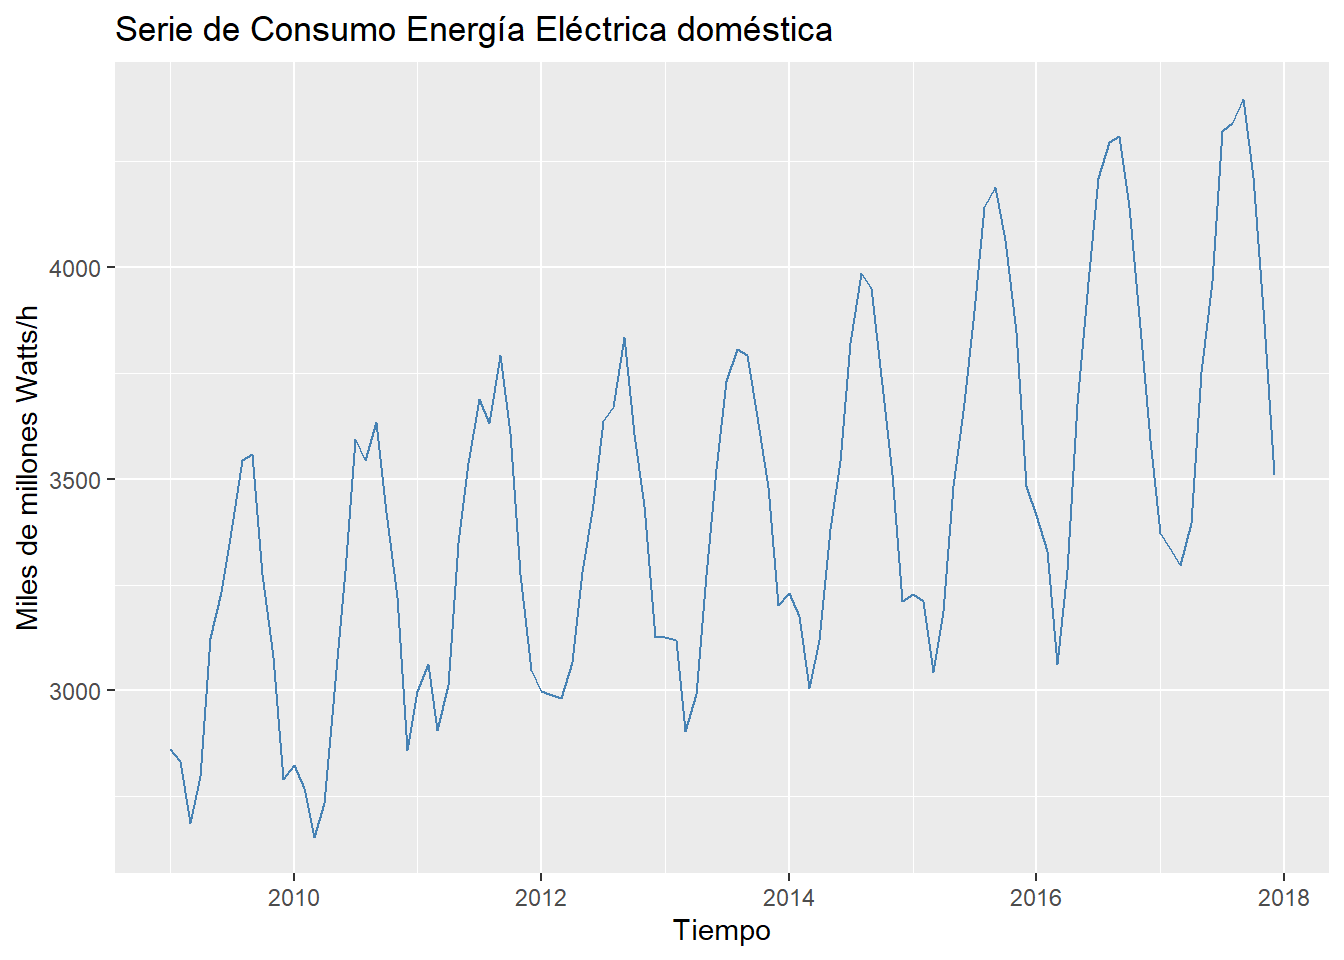
\includegraphics{TimeSeries_files/figure-latex/plotBaseSeries-1} 

}

\caption{Gráfica con ggplot usando programación nativa de R}\label{fig:plotBaseSeries}
\end{figure}

La gráfica \ref{fig:plotBaseSeries} es adecuada ya que usa una potente herramienta de graficación como lo es \emph{ggplot}, sin embargo, tuvo que crearse 3 diferentes objectos, una base de datos llamada \emph{CONELDO.base}, un vector donde se encuentran los valores de la serie de tiempo \_CONELDO \_y un vector que recibe el nombre de \emph{time} el cual contiene una secuencia de fechas. Si se usará el objeto time series (ts) estas declaraciones no serían necesarias pues en este objeto se indexa el tiempo, así en el siguiente código puede observar que el resultado es equivalente al observado en la gráfica \ref{fig:plotBaseSeries}.

\begin{Shaded}
\begin{Highlighting}[]
\FunctionTok{plot}\NormalTok{(CONELDO.ts,  }\AttributeTok{xlab=} \StringTok{\textquotesingle{}Tiempo\textquotesingle{}}\NormalTok{, }
     \AttributeTok{ylab =} \StringTok{\textquotesingle{}Miles de millones Watts/h\textquotesingle{}}\NormalTok{,}
     \AttributeTok{main =} \StringTok{\textquotesingle{}Serie de Consumo Energía Eléctrica doméstica\textquotesingle{}}\NormalTok{,}
     \AttributeTok{col=}\StringTok{\textquotesingle{}steelblue\textquotesingle{}}\NormalTok{)}
\end{Highlighting}
\end{Shaded}

\begin{figure}

{\centering 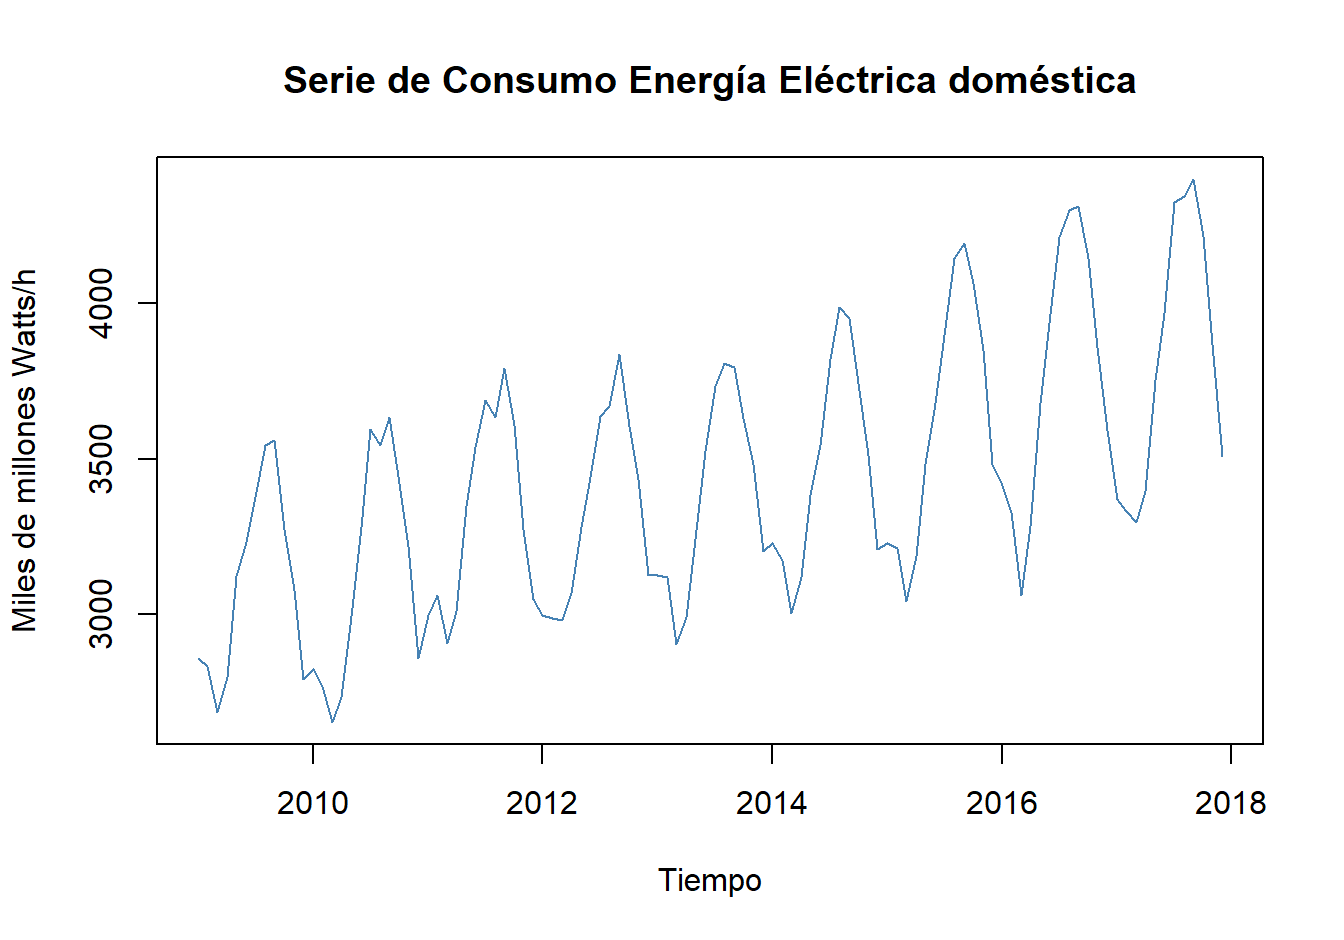
\includegraphics{TimeSeries_files/figure-latex/plotSerieCONELDO-1} 

}

\caption{Gráfica con plot usando el objeto ts}\label{fig:plotSerieCONELDO}
\end{figure}

Otra manera de poder graficar los datos a través de R es basándose en la librería \emph{xts}, este paquete incorpora una extensión al objeto \emph{ts} que viene por defecto en la instalación de R. El beneficio de \emph{xts} es que se pueden implementar varios tipos de gráficas auxiliares de series de tiempo, dentro del proceso de graficación ayuda a generar gráficas con un mayor control sobre los ejes además de añadir líneas en puntos de interés para ubicar mejor el tiempo y etiquetas más personalizadas. El proceso es similar al obtenido en la figura \ref{fig:plotSerieCONELDO}, sin embargo , es necesario convertir el objeto \textbf{ts} a uno \textbf{xts}, para ello se usará la función \emph{as.xts()}, además sobre la gráfica se añadirá la opción \emph{major.ticks} para añadir etiquetas en el eje de las \(X\) según lo indiquemos, dentro de este parámetro se pueden indicar especificar los siguientes valores, `auto',`minute', `hours', `days', `weeks', `months', `quarters', y `years', pare periodos, automático, minutos, horas, días, semanas, meses, trimestres y años, respectivamente.

\begin{Shaded}
\begin{Highlighting}[]
\FunctionTok{library}\NormalTok{(xts)}
\NormalTok{CONELDO.xts }\OtherTok{=} \FunctionTok{as.xts}\NormalTok{(CONELDO.ts)}

\FunctionTok{plot}\NormalTok{(CONELDO.xts, }\AttributeTok{col =} \StringTok{\textquotesingle{}steelblue\textquotesingle{}}\NormalTok{, }
     \AttributeTok{grid.ticks.on =} \StringTok{\textquotesingle{}quarters\textquotesingle{}}\NormalTok{, }\CommentTok{\#Crea líneas verticales sobre la gráfica cada trimestre}
     \AttributeTok{major.ticks =} \StringTok{\textquotesingle{}quarters\textquotesingle{}}\NormalTok{,  }\CommentTok{\#Crea líneas verticales sobre la gráfica cada trimestre}
     \AttributeTok{minor.ticks =}\StringTok{\textquotesingle{}years\textquotesingle{}}\NormalTok{, }\CommentTok{\# Escribe la etiqueta de los meses cada cierto tiempo}
     \AttributeTok{grid.col =} \StringTok{\textquotesingle{}lightgrey\textquotesingle{}}\NormalTok{, }\CommentTok{\#color líneas verticales}
     \AttributeTok{main=}\StringTok{\textquotesingle{}Serie de Consumo Energía Eléctrica doméstica\textquotesingle{}}
     
\NormalTok{     )}
\end{Highlighting}
\end{Shaded}

\begin{figure}

{\centering 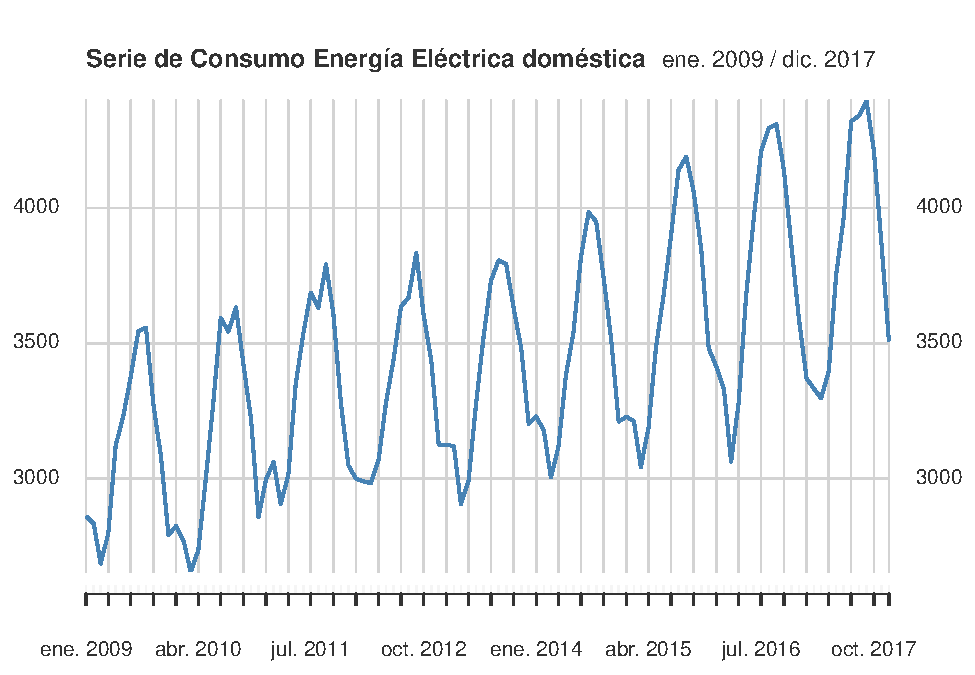
\includegraphics{TimeSeries_files/figure-latex/plotSeriexts-1} 

}

\caption{Gráfica con plot usando el objeto xts}\label{fig:plotSeriexts}
\end{figure}

Las gráficas que se acaban de realizar son adecuadas, sin embargo, cada una de ellas tiene sus ventajas y desventajas, desde luego no son las únicas formas de graficar series de tiempo en R existen otros paquetes externos dentro de la cual destaca \emph{zoo}. A pesar de ello, a lo largo de este texto se usará de manera indiferente cada uno de los tres métodos mostrados anteriormente, ya que son los más generales y destacan en los siguiente:

\begin{itemize}
\tightlist
\item
  La gráfica con \emph{ggplot2} (figura \ref{fig:plotBaseSeries}) es la gráfica más estética de las 3 que se acaban de realizar, sin embargo, aunque es muy personalizable la cantidad de código que hay que considerar es mayor que los otros dos métodos presentados. Además por la manera en que se programa dicha gráfica no admitirá el objeto \emph{ts}, por lo que se tiene que crear una tabla o \emph{data.frame} en la cual en una columna deberá ser almacenado el valor de la serie de tiempo, y en otra las fechas o tiempos en que ocurrió cada observación.
\item
  La gráfica usando el objeto \emph{ts} y \emph{plot()} (figura \ref{fig:plotSerieCONELDO}) es la gráfica más sencilla de implementar debido a que el comando \emph{plot()} acepta el objeto \emph{ts} y en dicha variable se encuentra indexado el tiempo, sólo será necesario indicar el nombre de las etiquetas y colores de la línea que sigue la serie de tiempo. El resultado es aceptable, sin embargo, estéticamente es la gráfica más sencilla de las presentadas anteriormente- Ya que no se tiene mucho control sobre las etiquetas del eje de las \(X\) y \(Y\) puede ocasionar que el lector se pierda en el tiempo y sea difícil comparar datos en un intervalo.
\item
  La gráfica usando el objeto \emph{xts} (figura \ref{fig:plotSeriexts}) es la más equilibrada de todas, el código es más sencillo y un poco menos vistosa que la gráfica \ref{fig:plotBaseSeries} usando \emph{ggplot} pero es más atractiva y ligeramente más elaborada que la gráfica \ref{fig:plotSerieCONELDO}. Al incorporar y controlar las líneas verticales en el eje de las \(X\) permite que el lector se ubique mejor en el tiempo y pueda comprar resultados. El aspecto negativo es que se tendrá que crear un nuevo objeto del tipo \emph{xts} lo cual consumirá un pequeño pero existente lugar en la memoria y espacio de trabajo.
\end{itemize}

Una vez seleccionado la gráfica que más beneficie al lector, la tarea subsecuente será analizar los datos en cuestión, se puede concluir que debido a las gráficas y en el resumen de la información, resultado de la función \emph{summary()}, la serie de tiempo tiene un valor mínimo de \(2,655\), máximo de \(4,398\) y medio de \(3,438\) mil millones Watts/hora, así mismo, en la gráfica de la serie de tiempo los datos presentan características comunes a muchas series económicas. Por ejemplo, es evidente que el \textbf{consumo de energía aumenta con el tiempo}, por lo que parece haber una clara \textbf{tendencia creciente}. También hay un ciclo evidente en los datos ya que se detecta una periodicidad anual, es decir, hay una clara \textbf{variación estacional} en los datos que da como resultado que en un año calendario los datos sean parecidos entre si en el mismo periodo de tiempo, como se puede llegar a apreciar, en todos los años el primer trimestre del año se tiene un consumo bajo de energía, después empieza a aumentar hasta alcanzar máximos locales a mediados de año y de ahí su consumo comienza a disminuir, dicho patrón se repite año con año por lo que se concluye que existe una periodicidad anual en la información.

La \textbf{comprensión de las causas probables} de las características de la serie puede formar una guía útil en el diseño y creación de un \textbf{modelo de serie de tiempo apropiado}. Para el caso particular de la serie CONELDO, las posibles causas que pueden incluir son:
* El aumento de la demanda de energía tiene una tendencia al alta pues el avance tecnológico y herramientas cada vez más sofisticadas hacen que el consumo eléctrico sea cada vez mayor.

\begin{itemize}
\tightlist
\item
  De igual forma, la tendencia al alta se puede deber a que existe en el país un crecimiento poblacional evidente y una mayor facilidad de adquisición de productos eléctricos.
\item
  El aumento de la demanda en ciertas épocas del año podría causarse debido a los períodos vacacionales, en específico a las de verano, ya que la serie al enfocarse al consumo eléctrico domestico esta temporada es cuando las personas pasan más tiempo en casa haciendo así que el consumo aumente.
\end{itemize}

Una gráfica de serie de tiempo no solo es importante para revelar patrones y características de los datos, sino que también puede revelar valores \textbf{atípicos potenciales o valores erróneos}, en inglés nombrados como \textbf{outliers}. Por ejemplo, los datos faltantes a veces se codifican con un valor negativo, como 0 o como valores ausentes (NA); obviamente, dichos valores tendrían que tratarse de manera diferente en el análisis, y ciertamente no querrían incluirse como observaciones al ajustar un modelo a los datos, así que habría que realizar técnicas de imputación de los datos para solucionar dichos problemas.

Para obtener una visión más clara de la tendencia, R incorpora funciones que tratan de estimar la tendencia realizando una media móvil centrada de orden relativo a la periodicidad de la información, más adelante se detallará este proceso, pero en este primer acercamiento se usará la función de \emph{aggregate()} para detectar gráficamente la tendencia sin el efecto de la periodicidad.

\begin{Shaded}
\begin{Highlighting}[]
\NormalTok{CONELDO.tendencia }\OtherTok{=} \FunctionTok{aggregate}\NormalTok{(CONELDO.ts)}
\FunctionTok{plot}\NormalTok{(CONELDO.tendencia, }\AttributeTok{col=}\StringTok{\textquotesingle{}steelblue\textquotesingle{}}\NormalTok{, }
    \AttributeTok{main=}\StringTok{\textquotesingle{}Tendencia del consumo eléctrico\textquotesingle{}}\NormalTok{,}
    \AttributeTok{xlab=} \StringTok{\textquotesingle{}Tiempo\textquotesingle{}}\NormalTok{,}
    \AttributeTok{ylab=}\StringTok{\textquotesingle{}Miles de Wats/h\textquotesingle{}}\NormalTok{)}
\end{Highlighting}
\end{Shaded}

\begin{figure}

{\centering 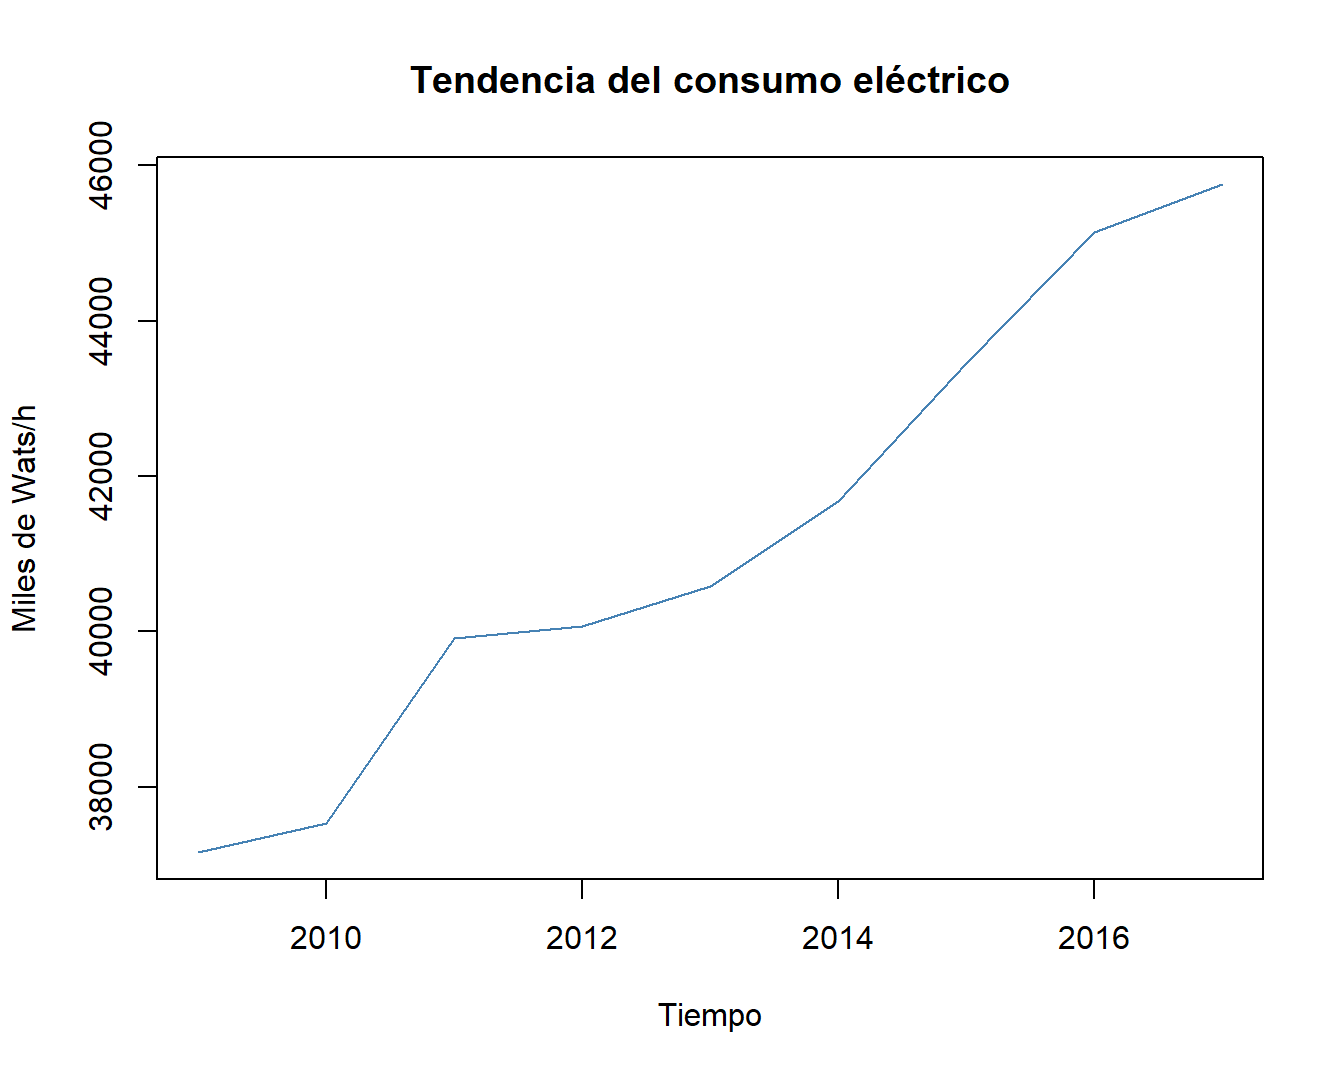
\includegraphics{TimeSeries_files/figure-latex/plotTendenciaCONELDO-1} 

}

\caption{Gráfica de la tendencia de la serie CONELDO}\label{fig:plotTendenciaCONELDO}
\end{figure}

Tal y como se observa en la gráfica \ref{fig:plotTendenciaCONELDO} existe una tendencia positiva, no es una tendencia lineal ya que existen aumentos significativos a lo largo del tiempo, pero a pesar de ello, la se serie nunca decrece en el tiempo en el periodo de observación, lo que refuerza al comentario hecho en los puntos anteriores.

De igual manera como sucede en el código anterior se puede poner especial atención a la periodicidad de la serie de tiempo, para ello se usará la función \emph{cycle} y \emph{boxplot} para elaborar gráficas de caja para cada mes y observar como es el desempeño de la serie de tiempo en dicha periodicidad. Si existiese una variación estacional entonces los patrones podrían ser fácilmente observado con ayuda del siguiente código.

\begin{Shaded}
\begin{Highlighting}[]
\FunctionTok{boxplot}\NormalTok{(CONELDO.ts }\SpecialCharTok{\textasciitilde{}} \FunctionTok{cycle}\NormalTok{(CONELDO.ts),}
        \AttributeTok{col =} \StringTok{"orange"}\NormalTok{, }\CommentTok{\# Color de relleno}
        \AttributeTok{border =} \StringTok{"brown"}\NormalTok{, }\CommentTok{\#Color de contorno}
        \AttributeTok{main=}\StringTok{\textquotesingle{}Consumo eléctrico doméstico\textquotesingle{}}\NormalTok{,}
        \AttributeTok{xlab=} \StringTok{\textquotesingle{}Tiempo\textquotesingle{}}\NormalTok{,}
        \AttributeTok{ylab=}\StringTok{\textquotesingle{}Miles de Wats/h\textquotesingle{}}\NormalTok{,}
        \AttributeTok{names =}\NormalTok{ month.abb }\CommentTok{\# Agregar nombres puede ser month.abb o month.name o }
                          \CommentTok{\#cualquier vector personalizado}
\NormalTok{        )}
\end{Highlighting}
\end{Shaded}

\begin{figure}

{\centering 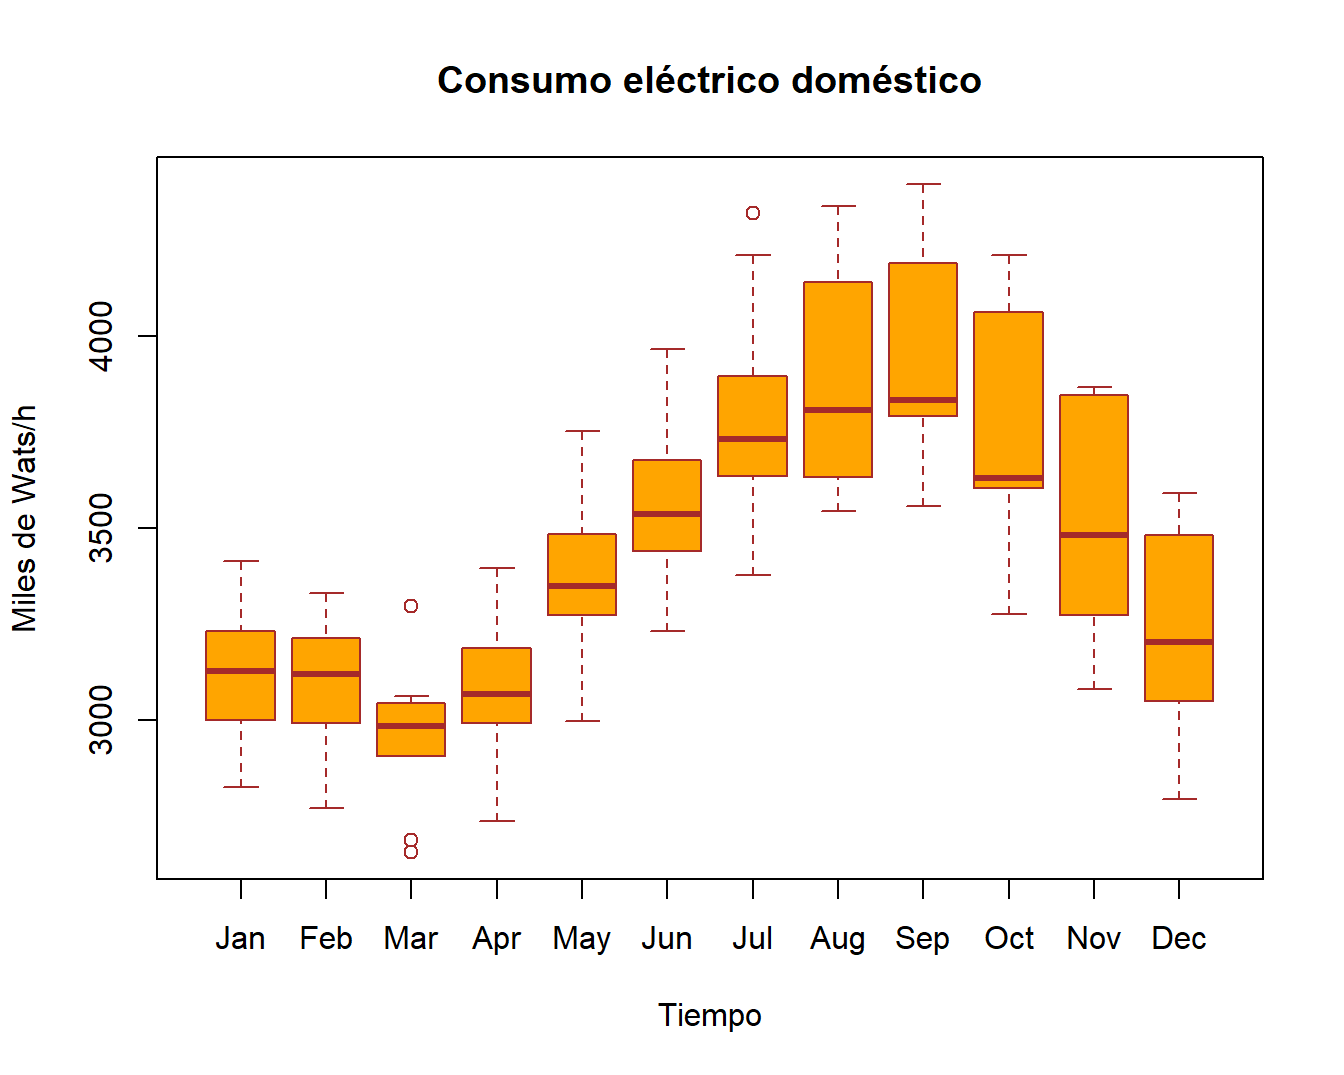
\includegraphics{TimeSeries_files/figure-latex/boxplotPeriodicidadCONELDO-1} 

}

\caption{Gráfica de la variación de la serie CONELDO}\label{fig:boxplotPeriodicidadCONELDO}
\end{figure}

Lo que realiza la gráfica de boxplot o de caja es reunir todos los valores de un mes determinado y comparar su distribución, el borde inferior de la caja corresponde al primer cuartil de los datos (el punto en el que se acumula el 25\% de los datos), la línea horizontal en la parte media corresponde a la mediana (donde se acumula el 50\% de las observaciones), y el borde superior de la caja corresponde al tercer cuartil (punto en el que se acumula el 75\% de los datos), hay que notar que la diferencia del tercer y primer cuartil corresponde a lo que se conoce como el rango intercuantil denotado como IQR. Las líneas que sobresalen de la caja y al final terminan con una pequeña línea horizontal corresponde a los valores máximos si esta sobre sale de la caja en la parte superior, mientras que la línea inferior corresponde al mínimo. Algunos meses cuentan con pequeños círculos que sobresalen las líneas mencionadas anteriormente, estos puntos son considerados valores atípicos u outliers, ya que son más chicos o más grande que \(\mbox{Primer Cuartil } -1.5 \ IQR\) o \(\mbox{Tercer Cuartil }+1.5 \ IQR\) respectivamente.

En la gráfica \ref{fig:boxplotPeriodicidadCONELDO} se observa que la serie tiene una clara variación estacional pues al agrupar cada mes se observa que: enero y febrero tienen un comportamiento similar, en marzo el consumo disminuye alcanzando los valores mínimos, a partir de este mes el consumo empieza a aumentar hasta alcanzar los topes máximos de consumo en el mes de septiembre para posteriormente disminuir paulatinamente hasta diciembre, estos mismos resultados se pueden visualizar en la siguiente gráfica de periodicidad.

\begin{Shaded}
\begin{Highlighting}[]
\FunctionTok{library}\NormalTok{(forecast)}

\FunctionTok{par}\NormalTok{(}\AttributeTok{mfrow=}\FunctionTok{c}\NormalTok{(}\DecValTok{1}\NormalTok{,}\DecValTok{2}\NormalTok{)) }\CommentTok{\#Permite graficar dos gráficas en una ventana}

\FunctionTok{ggseasonplot}\NormalTok{(CONELDO.ts,}
             \AttributeTok{polar=}\ConstantTok{FALSE}\NormalTok{, }
             \AttributeTok{main=}\StringTok{"Periodicidad del consumo de energía eléctrica"}\NormalTok{ )}

\FunctionTok{ggseasonplot}\NormalTok{(CONELDO.ts,}
             \AttributeTok{polar=}\ConstantTok{TRUE}\NormalTok{,}
             \AttributeTok{main=}\StringTok{"Periodicidad del consumo de energía eléctrica (Polar)"}\NormalTok{ )}

\FunctionTok{par}\NormalTok{(}\AttributeTok{mfrow=}\FunctionTok{c}\NormalTok{(}\DecValTok{1}\NormalTok{,}\DecValTok{1}\NormalTok{))}\CommentTok{\#Volvemos a iniciar la ventana }
\end{Highlighting}
\end{Shaded}

\begin{figure}

{\centering 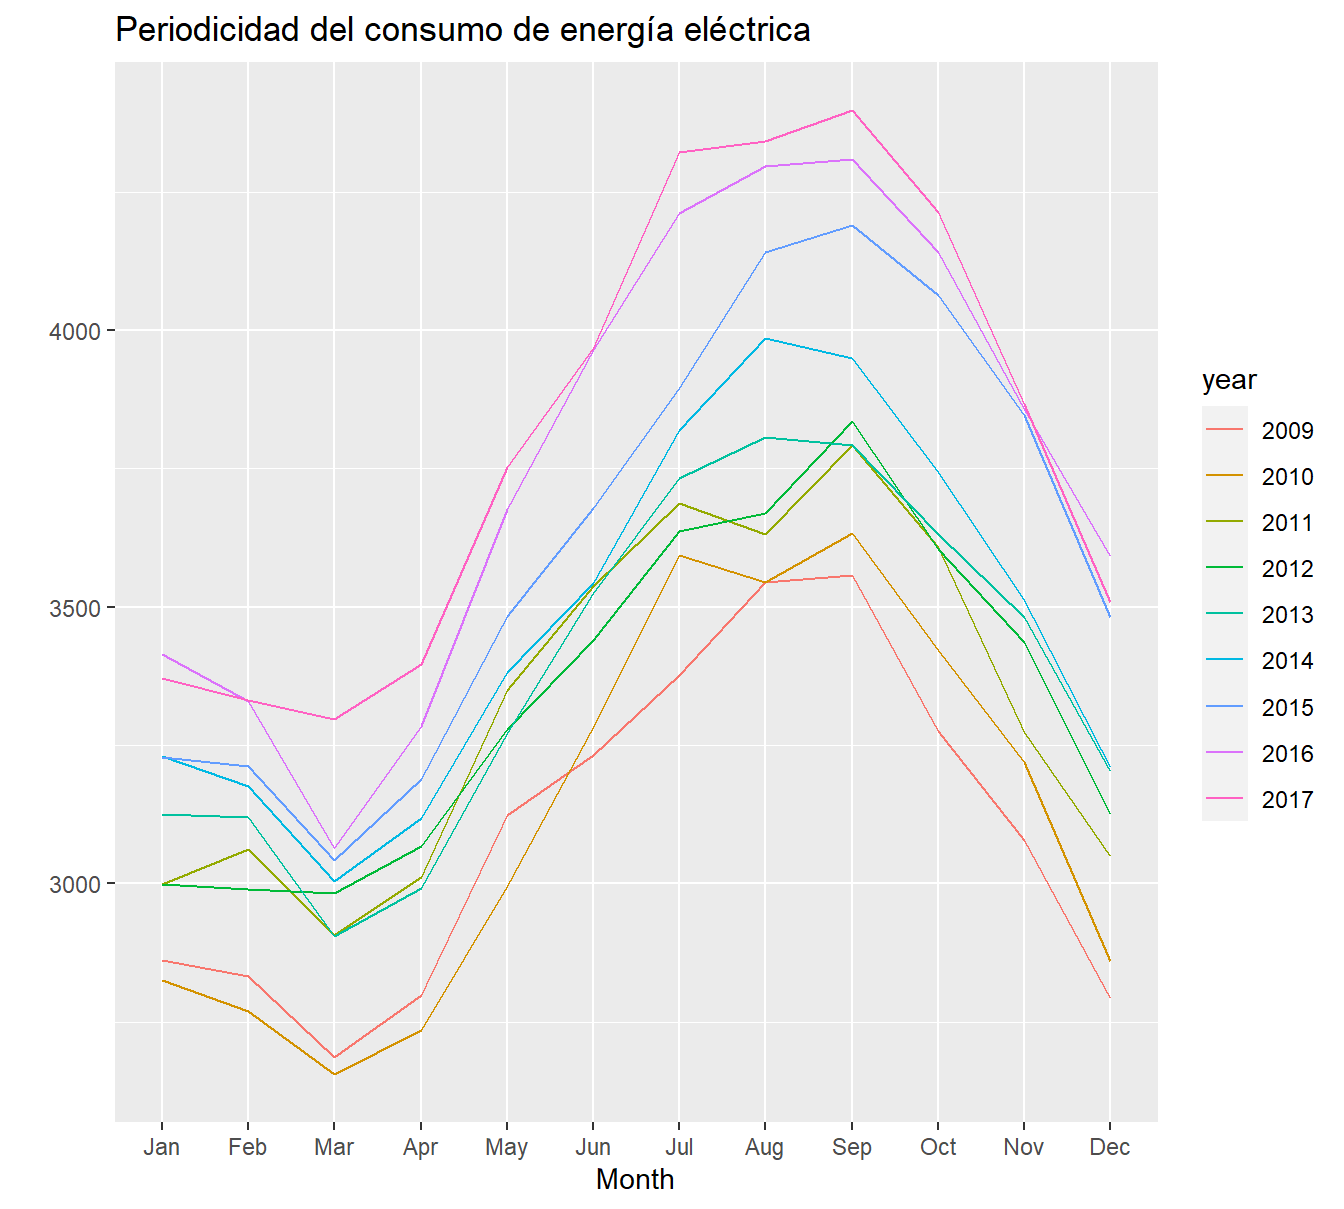
\includegraphics[width=0.5\linewidth]{TimeSeries_files/figure-latex/plotPeriodicidadCONELDO-1} 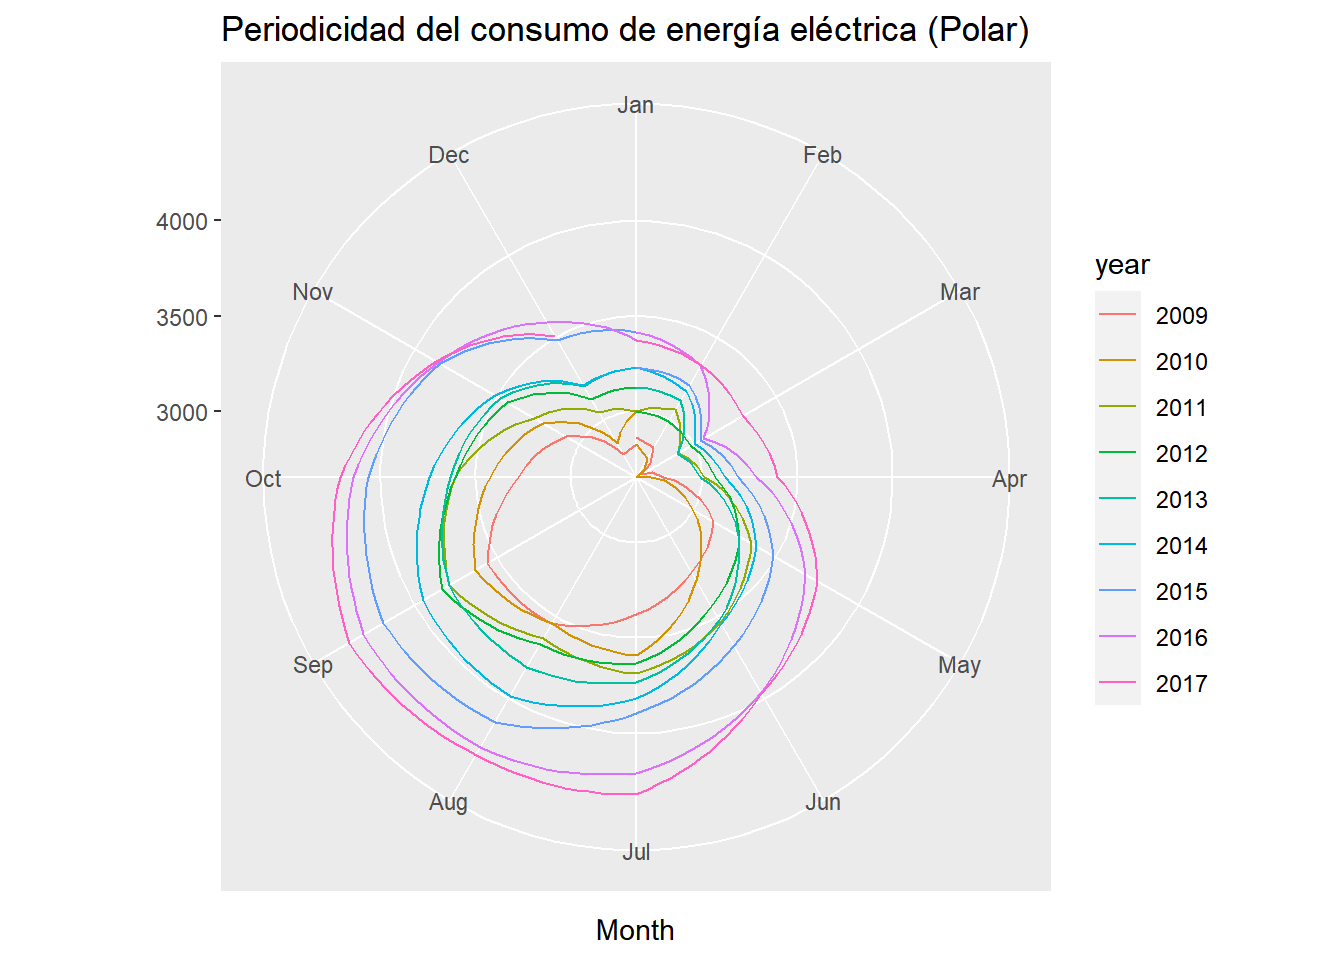
\includegraphics[width=0.5\linewidth]{TimeSeries_files/figure-latex/plotPeriodicidadCONELDO-2} 

}

\caption{Gráfica de la variación de la serie CONELDO por año}\label{fig:plotPeriodicidadCONELDO}
\end{figure}

A diferencia de la gráfica de caja donde se analizaban todos los años en conjunto, la función \emph{ggseasonplot} contenida en la paquetería \emph{forecast} y ejecutada en la gráfica \ref{fig:plotPeriodicidadCONELDO} permite detectar año con año los patrones que sigue la serie de tiempo, la gráfica de la izquierda se encuentra en un plano cartesiano, debido a que lo indicamos con la función \emph{polar = FALSE}, en ella se ve el incremento que ocurre año con año, pero también los patrones en el consumo, mientras que la gráfica de la derecha, al trabajar con una periodicidad anual permite particionar los datos e identificar los patrones más fácilmente, si la serie se comportará igual a lo largo del tiempo el resultado sería una gráfica completamente circular para cada periodo, sin embargo, en el caso particular del consumo de energía en México, se observa que el primer semestre del año hay un consumo menor comparado con la segunda mitad del año.

\hypertarget{variables-econuxf3micas-de-australia}{%
\subsection{Variables económicas de Australia}\label{variables-econuxf3micas-de-australia}}

El siguiente ejemplo que se analizará hace referencia a un objeto múltiple de series de tiempo y la importancia de formar este objeto cuando hay varias series referente a un mismo objeto de estudio. La base con la que se trabajará puede consultarse en el siguiente \href{https://raw.githubusercontent.com/omarr667/TimeSeries/main/Databases/cbe.dat.txt}{link}, dicha base de datos contiene una serie de variables económicas de Australia registrado del periodo de enero de 1958 a diciembre de 1990 obtenida de la Australian Bureau of Statistics. La base de datos contiene tres columnas, las primeras de ellas \emph{choc} y \emph{beer} que hace referencia a la producción de chocolate y cerveza en toneladas, mientras que \emph{elec} representa el consumo de energía eléctrica en millones de KW sobre hora.

Lo primero que debe realizar es importar de datos en la memoria y espacio de trabajo dentro de R, para ello, se debe de analizar el archivo que contiene los datos, la extensión y con ello elegir el método de importación que mejor se adapte. Debido a que el archivo descargado es del tipo \emph{dat} y dentro del archivo cada registro se encuentra separado por espacios lo más conveniente será utilizar la función \emph{read.table()} especificando como primer parámetro la ubicación del archivo y como segundo si la tabla contiene o no encabezados, puede observar los primeros 10 renglones en la tabla \ref{tab:australia}.

\begin{Shaded}
\begin{Highlighting}[]
\NormalTok{cbe.base }\OtherTok{=} \FunctionTok{read.table}\NormalTok{(}\StringTok{\textquotesingle{}Databases/cbe.dat\textquotesingle{}}\NormalTok{, }\CommentTok{\#Dirección del archivo}
          \AttributeTok{header=}\ConstantTok{TRUE}\NormalTok{) }\CommentTok{\#True si en el primer rengón se encuentran los encabezados}
\end{Highlighting}
\end{Shaded}

\begin{table}

\caption{\label{tab:australia}Variables económicas de Australia de 1958 a diciembre de 1990 }
\centering
\begin{tabular}[t]{rrr}
\toprule
choc & beer & elec\\
\midrule
1451 & 96.3 & 1497\\
2037 & 84.4 & 1463\\
2477 & 91.2 & 1648\\
2785 & 81.9 & 1595\\
2994 & 80.5 & 1777\\
\addlinespace
2681 & 70.4 & 1824\\
3098 & 74.8 & 1994\\
2708 & 75.9 & 1835\\
2517 & 86.3 & 1787\\
2445 & 98.7 & 1699\\
\bottomrule
\end{tabular}
\end{table}

Siguiendo la estandarización en el análisis de series de tiempo observado en el ejemplo \ref{coneldo}, un punto fundamental es la realización de gráficas para apreciar el contenido de este, para ello se creará gráficas por medio de \emph{ggplot}, \emph{xts} y con la programación básica de R por medio de \emph{ts}.

Para realizar gráficas con \emph{ggplot} será necesario usar una estructura de base de datos siguiendo la estandarización de \textbf{tidy}. Una estructura de base de datos \textbf{tidy} es importante en R, pues muchos paquetes están construidos para este tipo de estructura, tal es el caso de \emph{ggplot}, para ello, R cuenta con herramientas para facilitar la conversión de tablas de una estructura clásica a una del tipo \textbf{tidy}. Una tabla de la forma clásica tiene una estructura similar a la tabla \ref{tab:australia}, en donde cada columna contiene una variable de interés, y cada renglón a una observación por ejemplo, la producción de chocolate y cerveza en un periodo se muestra en un mismo renglón pero en diferente columna. Sin embargo, una estructura siguiendo la metodología \textbf{tidy} lo que propone es que el conjunto de datos sea ordenado siguiendo las siguientes \href{https://cran.r-project.org/web/packages/tidyr/vignettes/tidy-data.html}{reglas}:

\begin{itemize}
\tightlist
\item
  Las cabeceras de las columnas son valores, no nombres de variables.
\item
  Se almacenan múltiples variables en una columna.
\item
  Las variables se almacenan tanto en filas como en columnas.
\item
  Se almacenan múltiples tipos de unidades de observación en la misma tabla.
\item
  Una misma unidad de observación se almacena en varias tablas.
\end{itemize}

De esta manera, la tabla de variables económicas siguiendo esta metodología, pasa de un enfoque clásico como \ref{tab:australia} a uno ordenado bajo \textbf{tidy} de la forma \ref{tab:australiatidy}.

\begin{Shaded}
\begin{Highlighting}[]
\FunctionTok{library}\NormalTok{(dplyr) }\CommentTok{\#Libreria de manejo de datos}
\FunctionTok{library}\NormalTok{(tidyr) }\CommentTok{\#Libreria auxliar para convertir base a tidy}

\NormalTok{cbe.base.tidy }\OtherTok{=}\NormalTok{ cbe.base }\SpecialCharTok{\%\textgreater{}\%}  \CommentTok{\#base de donde sacamos información}
  \FunctionTok{mutate}\NormalTok{(}\AttributeTok{time =}      \CommentTok{\#Creamos una variable que se llame time}
           \FunctionTok{as.Date}\NormalTok{(  }\CommentTok{\#Por defecto es una secuencia del timpo datetime, así que convertimos a Date}
                \FunctionTok{seq}\NormalTok{(}\FunctionTok{ISOdate}\NormalTok{(}\DecValTok{1958}\NormalTok{,}\DecValTok{01}\NormalTok{,}\DecValTok{01}\NormalTok{),  }\CommentTok{\#secuencia, fecha inicial}
                \FunctionTok{ISOdate}\NormalTok{(}\DecValTok{1990}\NormalTok{,}\DecValTok{12}\NormalTok{,}\DecValTok{01}\NormalTok{),  }\CommentTok{\#Fecha final }
                \AttributeTok{by =} \StringTok{"month"}\NormalTok{) }\CommentTok{\# cantidad de incremento}
\NormalTok{                )  }
\NormalTok{         ) }\SpecialCharTok{\%\textgreater{}\%} \CommentTok{\#Pasamos la \textquotesingle{}nueva base\textquotesingle{} a la opción gather para convertir a tidy}
  \FunctionTok{gather}\NormalTok{(}\AttributeTok{key=}\StringTok{\textquotesingle{}serie\textquotesingle{}}\NormalTok{,  }\CommentTok{\#Columna a crear donde se almacenan las variables}
         \AttributeTok{value=}\StringTok{\textquotesingle{}Produccion\textquotesingle{}}\NormalTok{, }\CommentTok{\#columna donde se almacena el valor de la variable }
         \DecValTok{1}\SpecialCharTok{:}\DecValTok{3}\NormalTok{) }\SpecialCharTok{\%\textgreater{}\%} \CommentTok{\#Columnas a transponer}
  \FunctionTok{arrange}\NormalTok{(time)  }\CommentTok{\# ordenamos los datos por fecha}
\FunctionTok{head}\NormalTok{(cbe.base.tidy, }\DecValTok{10}\NormalTok{)}
\end{Highlighting}
\end{Shaded}

\begin{table}

\caption{\label{tab:australiatidy}Variables económicas de Australia de 1958 a diciembre de 1990 }
\centering
\begin{tabular}[t]{llr}
\toprule
time & serie & Produccion\\
\midrule
1958-01-01 & choc & 1451.0\\
1958-01-01 & beer & 96.3\\
1958-01-01 & elec & 1497.0\\
1958-02-01 & choc & 2037.0\\
1958-02-01 & beer & 84.4\\
\addlinespace
1958-02-01 & elec & 1463.0\\
1958-03-01 & choc & 2477.0\\
1958-03-01 & beer & 91.2\\
1958-03-01 & elec & 1648.0\\
1958-04-01 & choc & 2785.0\\
\bottomrule
\end{tabular}
\end{table}

La tabla \ref{tab:australiatidy}, fue creada utilizando dplyr, y tidyr ya que son librerías muy versátiles para el manejo de datos y sumamente amplias por lo que sólo se comentará las funciones empleadas, el lector que lo desee puede aprender más sobre el tema en la introducción oficial contenida en el siguiente \href{https://cran.r-project.org/web/packages/dplyr/vignettes/dplyr.html}{link}. Dplyr y tidyr forman parte de una gran serie de paquetes que en conjunto son llamados \emph{tidyverse}. Dplyr es la raíz de la programación de este tipo de funciones, aunque en primera instancia destaca la cantidad de código que se ha de implementar, este conjunto de funciones está diseñado para permitir la manipulación de datos de una manera intuitiva y fácil de usar, cada función que se invoca debe ser seguida con el operador denominado \emph{pipe} el cual se denota como \(\%>\%\) Las funciones más importantes contenidas en diplyr son las siguientes:

\begin{itemize}
\tightlist
\item
  \emph{select()}, función que recibe como parámetros todas las columnas con las que se realizará un subconjunto de la tabla original, es decir, como dice su nombre selecciona las columnas de base principal.
\item
  \emph{filter()}, función que recibe una condición dada por el usuario para filtrar la información que cumple dicha condición.
\item
  \emph{arrange()}, permite ordenar el data.frame bajo la columna o columnas indicadas.
\item
  \emph{mutate()}, permite la creación de nueva columna, ya sea a través de valores contantes u operaciones entre columnas.
  *\emph{group by()}, permite especificar las columnas que se van a agrupar, para que dentro de esta agrupación se ejecute operación de resumen.
\item
  \emph{summarize()}, permite resumir la información de una variable respecto a la agrupación hecha en el punto anterior, por ejemplo, puede agruparse los datos por una variable de interés y sobre otra. conocer la suma, conteo, valores máximo o mínimos sobre la variable de agrupación.
\item
  \emph{gather()}, función dentro de tidyr que permite transponer los datos para transformar de una tabla clásica a una tabla tidyr.
\item
  \emph{spread()}, función dentro de tidyr, que permite transponer los datos para transformar una tabla tidyr a una clásica.
\end{itemize}

Quien conozca programación en SQL muchas de las funciones mostradas le serán muy familiares, pues al final este es uno de los objetivos de \textbf{dplyr}, heredar la idea lógica de la programación SQL para que esta sea adaptada en R y permitir un manejo de datos adecuado.

Es importante transformar los datos de una serie con enfoque clásico a uno con enfoque \emph{tidy}, ya que muchos de los análisis o procedimientos precargados en R se basan en tablas con esta estructura. Adaptar los datos a este formato requiere un trabajo inicial, pero ese trabajo vale la pena a largo plazo, el ejemplo puede observarse en la grafica \ref{fig:ggplotAustralia} la cual fue generada con el siguiente código:

\begin{Shaded}
\begin{Highlighting}[]
\FunctionTok{ggplot}\NormalTok{(cbe.base.tidy, }\FunctionTok{aes}\NormalTok{(}\AttributeTok{x=}\NormalTok{time, }\AttributeTok{y=}\NormalTok{Produccion, }\AttributeTok{color=}\NormalTok{serie)) }\SpecialCharTok{+}
  \FunctionTok{geom\_line}\NormalTok{()}
\end{Highlighting}
\end{Shaded}

\begin{figure}

{\centering 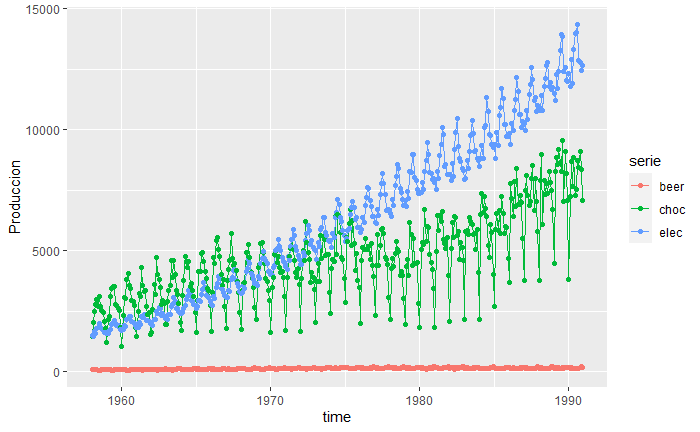
\includegraphics{Images/electric_ggplot} 

}

\caption{Gráfica sobre el consumo de electricidad y producción de cerveza y chocolate en Australia}\label{fig:ggplotAustralia}
\end{figure}

Como se aprecia en la figura \ref{fig:ggplotAustralia}, en un mismo diagrama se encuentran graficadas las tres series de tiempo, el problema que se presenta es que aunque se pueden mover los ejes para observar mejor el flujo de la información las cantidades no están en la misma escala es por ello que la producción de cerveza no se puede apreciar de la manera correcta, sin embargo, se puede notar, que aunque no se pueden comprar pues son unidades de medida completamente diferente al menos porcentualmente, la producción de chocolate se ha estancado a diferencia del consumo de energía eléctrica que ha tenido un crecimiento constante.

Debido a que se tiene la información en un formato \textbf{tidy}, el código puede ser modificado rápidamente para poder retratar de mejor manera las series de tiempo. Por el error observado anteriormente, ahora no interesaría graficar las tres series en una misma gráfica si no generar tres gráficas independientes en la que se pueda apreciar el comportamiento tal como se obtiene en la grafica \ref{fig:ggplotAustralia2}.

\begin{Shaded}
\begin{Highlighting}[]
\FunctionTok{ggplot}\NormalTok{(cbe.base.tidy, }\FunctionTok{aes}\NormalTok{(}\AttributeTok{x=}\NormalTok{time, }\AttributeTok{y=}\NormalTok{Produccion, }\AttributeTok{color=}\NormalTok{serie)) }\SpecialCharTok{+}
  \FunctionTok{geom\_line}\NormalTok{()}\SpecialCharTok{+}
  \FunctionTok{facet\_wrap}\NormalTok{(}\SpecialCharTok{\textasciitilde{}}\NormalTok{serie,   }\CommentTok{\#Realiza una gráfica por cada serie }
             \AttributeTok{scales  =} \StringTok{\textquotesingle{}free\textquotesingle{}}\NormalTok{,  }\CommentTok{\#Inidica que las escalas sean libres para cada gráfica}
             \AttributeTok{ncol=}\DecValTok{1}\NormalTok{) }\CommentTok{\#Número de columnas en la gráfica final }
\end{Highlighting}
\end{Shaded}

\begin{figure}

{\centering 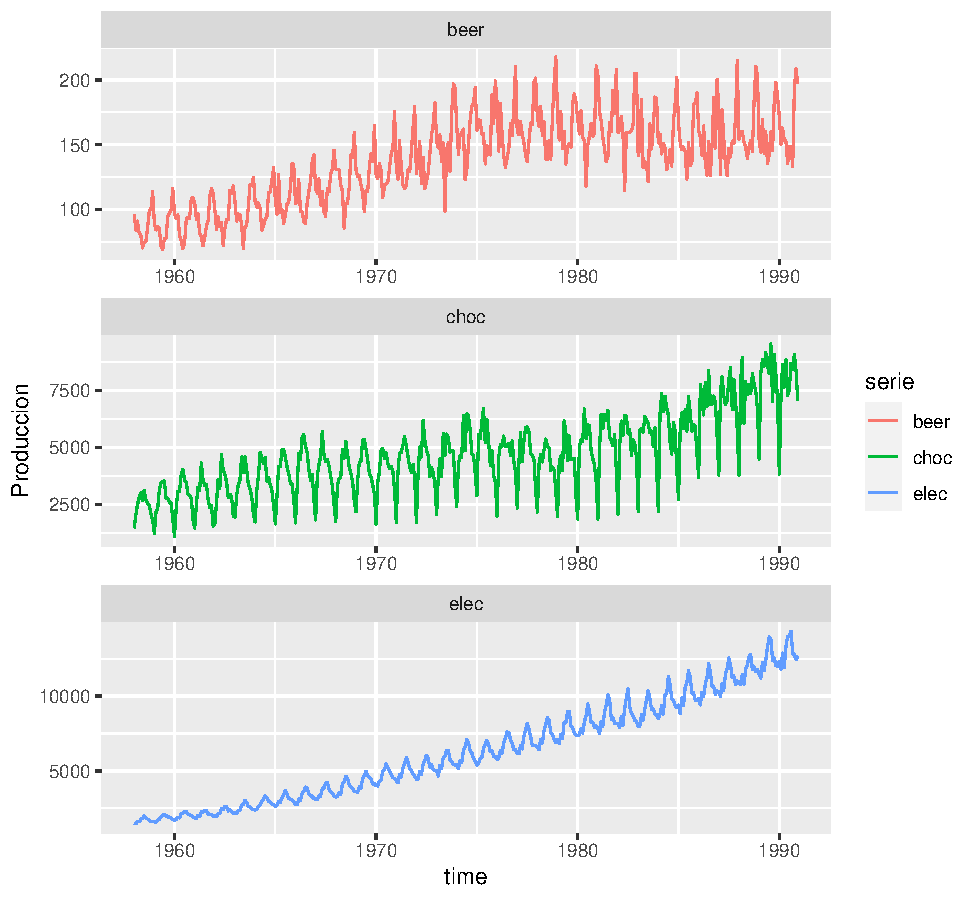
\includegraphics{TimeSeries_files/figure-latex/ggplotAustralia2-1} 

}

\caption{Gráfica sobre el consumo de electricidad y producción de cerveza y chocolate en Australia}\label{fig:ggplotAustralia2}
\end{figure}

Tal como ocurrió en el ejemplo de la sección anterior \ref{coneldo}, la cantidad de código y conceptos que hubo que emplear fue bastante con \emph{ggplot}, sin embargo, el resultado visualmente es excelente, ya que si el lector se encuentra interesado en graficar puede copiar las funciones y sólo cambiar los aspectos estéticos dando resultados a la medida de las necesidades. Aunque \emph{ggplot} es bueno para reportes posiblemente en la practica necesite resultados más inmediatos y no tan estéticos pues sería una primera fase de análisis. Debido a esta razón puede crear objetos de series de tiempo independientes para posteriormente unirlos en un objeto múltiple. La ventaja de esta labor es que cada comando o función que sea empleada serán aplicadas en todas las series contenidas en este objeto de series de tiempo múltiple.

Siguiendo entonces esta metodología, lo primero que se deberá de realizar, es convertir cada columna de la base \emph{cbe.base} a objetos de series de tiempo. Se sabe que cada secuencia de datos fue recopilada de manera mensual de enero de 1958 a diciembre de 1990, así que estas consideraciones deberán ser ingresadas como parámetro en la función \emph{ts()}. Una vez que se tengan las tres series de tiempo creadas, se usará la función \emph{ts.intersect()} para crear un objeto de serie de tiempo múltiple.

\begin{Shaded}
\begin{Highlighting}[]
\NormalTok{elec.ts }\OtherTok{=} \FunctionTok{ts}\NormalTok{(cbe.base}\SpecialCharTok{$}\NormalTok{elec, }\AttributeTok{start=}\DecValTok{1958}\NormalTok{, }\AttributeTok{freq=}\DecValTok{12}\NormalTok{) }\CommentTok{\#Creación de la serie elec}
\NormalTok{beer.ts }\OtherTok{=} \FunctionTok{ts}\NormalTok{(cbe.base}\SpecialCharTok{$}\NormalTok{beer, }\AttributeTok{start=}\DecValTok{1958}\NormalTok{, }\AttributeTok{freq=}\DecValTok{12}\NormalTok{) }\CommentTok{\#Creación de la serie beer}
\NormalTok{choc.ts }\OtherTok{=} \FunctionTok{ts}\NormalTok{(cbe.base}\SpecialCharTok{$}\NormalTok{choc, }\AttributeTok{start=}\DecValTok{1958}\NormalTok{, }\AttributeTok{freq=}\DecValTok{12}\NormalTok{) }\CommentTok{\#Creación de la serie choc}
\CommentTok{\#Se crea el objeto de serie de tiempo multiple}
\NormalTok{cbe.ts }\OtherTok{=} \FunctionTok{ts.intersect}\NormalTok{(elec.ts, beer.ts, choc.ts)}

\FunctionTok{head}\NormalTok{(cbe.ts, }\DecValTok{10}\NormalTok{) }\CommentTok{\#se imprimen los primeros 10 renglones}
\end{Highlighting}
\end{Shaded}

\begin{verbatim}
##          elec.ts beer.ts choc.ts
## Jan 1958    1497    96.3    1451
## Feb 1958    1463    84.4    2037
## Mar 1958    1648    91.2    2477
## Apr 1958    1595    81.9    2785
## May 1958    1777    80.5    2994
## Jun 1958    1824    70.4    2681
## Jul 1958    1994    74.8    3098
## Aug 1958    1835    75.9    2708
## Sep 1958    1787    86.3    2517
## Oct 1958    1699    98.7    2445
\end{verbatim}

Crear esta intersección de series de tiempo es muy importante ya que como los datos tienen una misma periodicidad todas las funciones de resumen puede ser empleadas sobre este objeto y no sobre las múltiples series de tiempo, por ejemplo, se puede consultar la clase del objeto que se acaba de crear, dando como resultado que es una matriz de serie de tiempo (mts), de igual manera, se obtiene el inicio, fin y frecuencia de la serie de tiempo, y la función \emph{summary} es capaz de resumir la información para cada serie proporcionando los valores mínimos, cuartiles y media.

\begin{Shaded}
\begin{Highlighting}[]
\FunctionTok{class}\NormalTok{(cbe.ts)}\CommentTok{\#El formato de la serie de tiempo es}
\end{Highlighting}
\end{Shaded}

\begin{verbatim}
## [1] "mts"    "ts"     "matrix"
\end{verbatim}

\begin{Shaded}
\begin{Highlighting}[]
\FunctionTok{start}\NormalTok{(cbe.ts)}\CommentTok{\#El incio de la serie de tiempo es}
\end{Highlighting}
\end{Shaded}

\begin{verbatim}
## [1] 1958    1
\end{verbatim}

\begin{Shaded}
\begin{Highlighting}[]
\FunctionTok{end}\NormalTok{(cbe.ts) }\CommentTok{\#Último perido donde se almacena información}
\end{Highlighting}
\end{Shaded}

\begin{verbatim}
## [1] 1990   12
\end{verbatim}

\begin{Shaded}
\begin{Highlighting}[]
\FunctionTok{frequency}\NormalTok{(cbe.ts)}\CommentTok{\#La frecuencia de la serie de tiempo es}
\end{Highlighting}
\end{Shaded}

\begin{verbatim}
## [1] 12
\end{verbatim}

\begin{Shaded}
\begin{Highlighting}[]
\FunctionTok{summary}\NormalTok{(cbe.ts) }\CommentTok{\#Información de la distribución de los datos}
\end{Highlighting}
\end{Shaded}

\begin{verbatim}
##     elec.ts         beer.ts         choc.ts    
##  Min.   : 1463   Min.   : 69.2   Min.   :1066  
##  1st Qu.: 3239   1st Qu.:113.7   1st Qu.:3460  
##  Median : 5891   Median :140.6   Median :4579  
##  Mean   : 6312   Mean   :137.6   Mean   :4685  
##  3rd Qu.: 8820   3rd Qu.:159.7   3rd Qu.:5735  
##  Max.   :14338   Max.   :217.8   Max.   :9558
\end{verbatim}

Esta construcción también es útil ya que permite la generación de gráficas más sencillas utilizado la programación nativa de R. Al indexar el tiempo, simplemente se ejecuta la opción \emph{plot()}, se añade el objeto de serie de tiempo múltiple y de manera opcional puede modificar algunos aspectos gráficos, dando como resultado la gráfica \ref{fig:plotAustraliats}.

\begin{Shaded}
\begin{Highlighting}[]
\FunctionTok{plot}\NormalTok{(cbe.ts, }
     \AttributeTok{main=} \StringTok{\textquotesingle{}Consumo de electricidad, de cerveza y chocolate en Australia\textquotesingle{}}\NormalTok{,}
     \AttributeTok{xlab=} \StringTok{\textquotesingle{}Tiempo\textquotesingle{}}\NormalTok{,}
     \AttributeTok{col =} \StringTok{\textquotesingle{}steelblue\textquotesingle{}}\NormalTok{)}
\end{Highlighting}
\end{Shaded}

\begin{figure}

{\centering 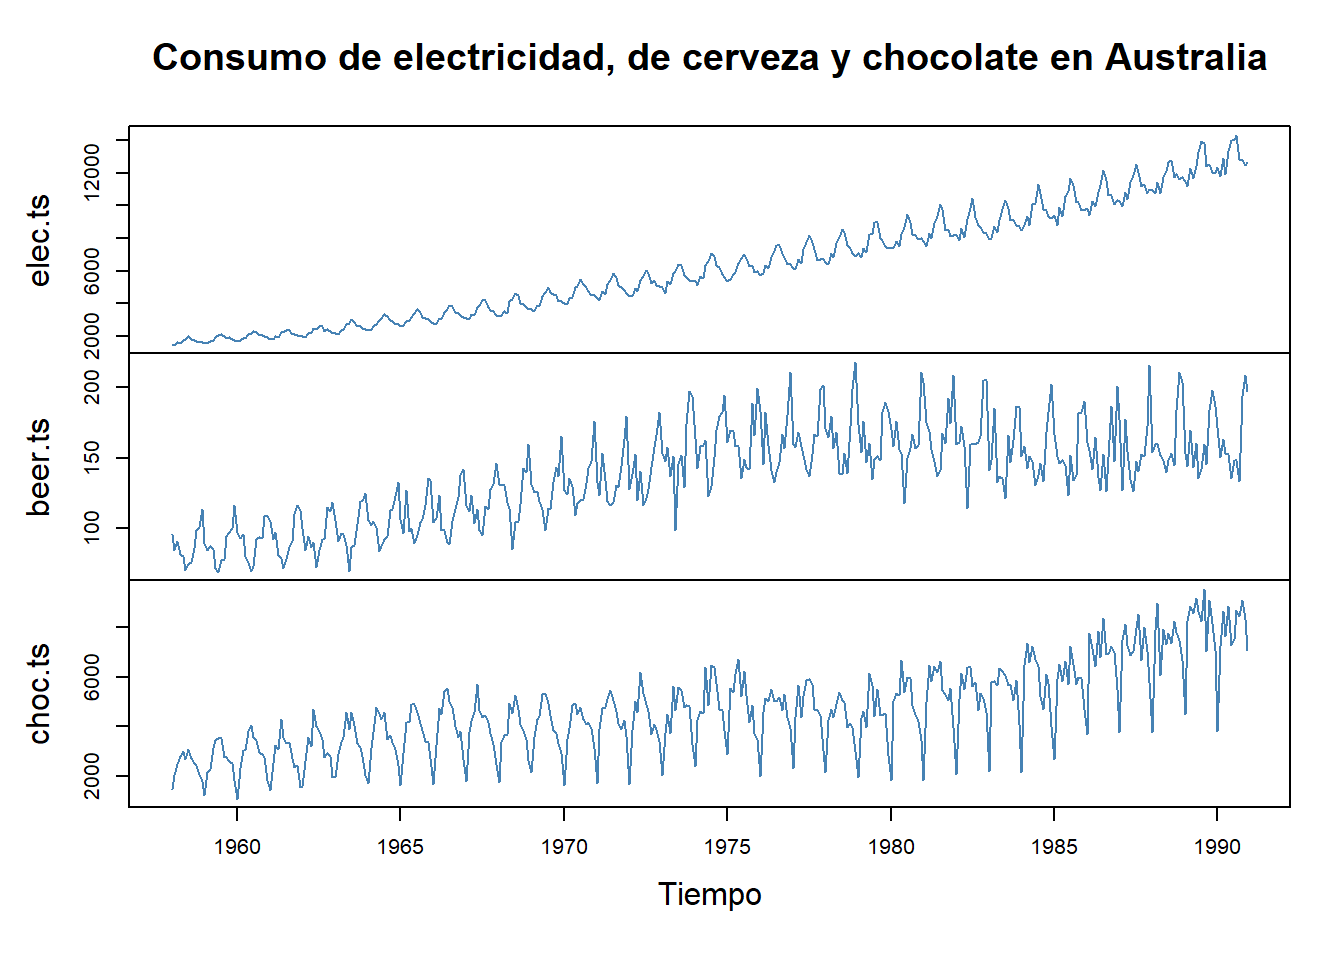
\includegraphics{TimeSeries_files/figure-latex/plotAustraliats-1} 

}

\caption{Gráfica sobre el consumo de electricidad y producción de cerveza y chocolate en Australia}\label{fig:plotAustraliats}
\end{figure}

De igual manera, pueden generarse gráficas utilizando el objeto \emph{xts}, recordar que esta clase puede heredar al objeto \emph{ts} por lo que sólo se tiene que especificar la transformación de dicho objeto con \emph{as.xts()}. Una vez transformada la variable, sólo se hará uso de la función \emph{plot()}, en este caso añadimos ciertos parámetros para hacer la gráfica equivalente a las figuras \ref{fig:ggplotAustralia2} y \ref{fig:plotAustraliats}, en caso de no añadir los últimos códigos el resultado será equivalente a la figura \ref{fig:ggplotAustralia2}.

\begin{Shaded}
\begin{Highlighting}[]
\NormalTok{cbe.xts }\OtherTok{=} \FunctionTok{as.xts}\NormalTok{(cbe.ts)}
\FunctionTok{plot}\NormalTok{(cbe.xts, }
     \AttributeTok{main=} \StringTok{\textquotesingle{}Consumo de electricidad, de cerveza y chocolate en Australia\textquotesingle{}}\NormalTok{,}
     \AttributeTok{xlab=} \StringTok{\textquotesingle{}Tiempo\textquotesingle{}}\NormalTok{,}
      \AttributeTok{multi.panel =} \DecValTok{3}\NormalTok{, }\CommentTok{\# Para generar 3 paneles (de lo contarario el resultado sería a ggplot)}
     \AttributeTok{yaxis.same =} \ConstantTok{FALSE}\NormalTok{) }\CommentTok{\#Para que los ejes se adapten a cada serie}
\end{Highlighting}
\end{Shaded}

\begin{figure}

{\centering 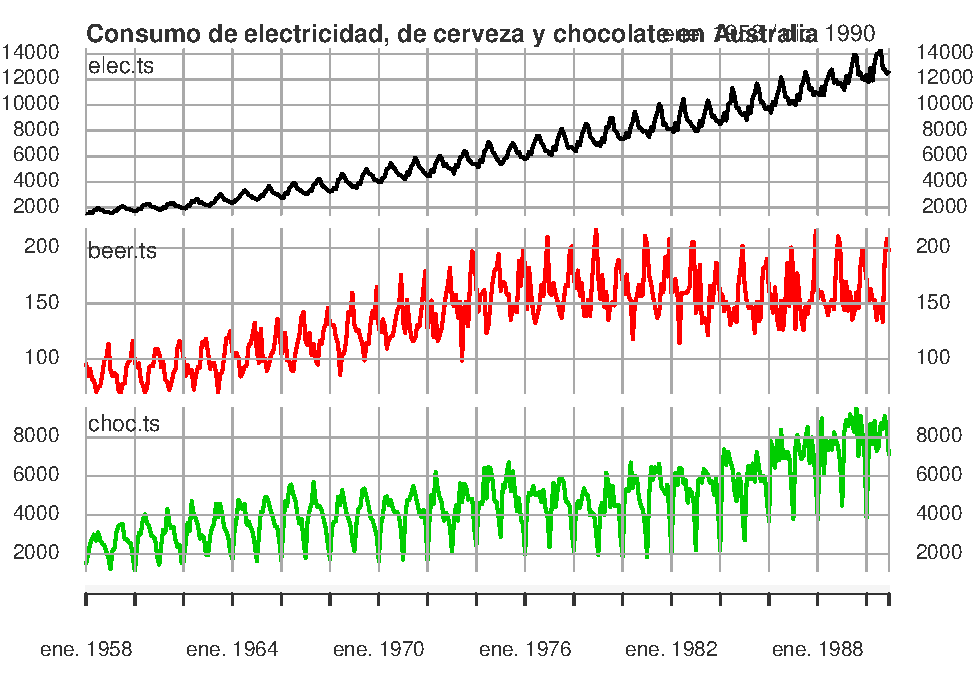
\includegraphics{TimeSeries_files/figure-latex/plotAustraliaxts-1} 

}

\caption{Gráfica sobre el consumo de electricidad y producción de cerveza y chocolate en Australia}\label{fig:plotAustraliaxts}
\end{figure}

Tal como se mencionó en la sección \ref{coneldo}, el lector puede elegir el método que mejor se adapte a sus necesidades, sin embargo, lo más recomendable es usar el objeto \emph{xts} ya que este tipo de gráficas se encuentran equilibradas, la cantidad de código no es excesiva y visualmente son presentables.

De las gráficas \ref{fig:ggplotAustralia2}, \ref{fig:plotAustraliats}, \ref{fig:plotAustraliaxts} puede observarse que las series tienen tendencias muy variadas; la primera, el consumo de electricidad tiene una clara ciclicidad y tendencia positiva que se comporta prácticamente lineal a lo largo del tiempo. Sin embargo, en la producción de chocolate y cerveza se observa una variación estacional que se repite a lo largo del tiempo, sin embargo, su tendencia aunque es positiva hay periodos en los que prácticamente se comporta de manera constante.

También se puede ver gráficamente que existe una correlación muy alta entre el consumo de electricidad y la producción de chocolate, es decir, si una aumenta la otra lo hace en una proporción muy parecida, por lo que las series a estimar debería de involucrar una correlación parecida es por ello por lo que las dos gráficas tienen un aspecto similar. Sin embargo, es importante tener en cuenta que esta correlación es engañosa y no puede establecer una causalidad ya que, aunque los dos involucran a aspectos de Australia no hay una clara relación de que el aumentar la producción de chocolate la producción aumente en la misma proporción, a este tipo de correlaciones se llaman relaciones espurias; La correlación existe porque ambos conjuntos de datos tienen una tendencia subyacente y una variación estacional. Cualquier serie que tenga una tendencia tenderá a estar correlacionada con cualquier otra serie que tenga tendencia parecida. Por esta razón, es preferible eliminar las tendencias y los efectos estacionales antes de comparar varias series.

\begin{Shaded}
\begin{Highlighting}[]
\FunctionTok{library}\NormalTok{(corrplot) }\CommentTok{\#Librería para gráficar correlaciones}
\end{Highlighting}
\end{Shaded}

\begin{verbatim}
## corrplot 0.90 loaded
\end{verbatim}

\begin{Shaded}
\begin{Highlighting}[]
\NormalTok{cbe.matrix }\OtherTok{=} \FunctionTok{cor}\NormalTok{(cbe.ts) }\CommentTok{\#Correlaciones}
\FunctionTok{corrplot.mixed}\NormalTok{(cbe.matrix, }\AttributeTok{lower.col=}\StringTok{"black"}\NormalTok{, }\AttributeTok{upper=}\StringTok{"color"}\NormalTok{) }\CommentTok{\#gráfica de correlaciones}
\end{Highlighting}
\end{Shaded}

\begin{figure}

{\centering 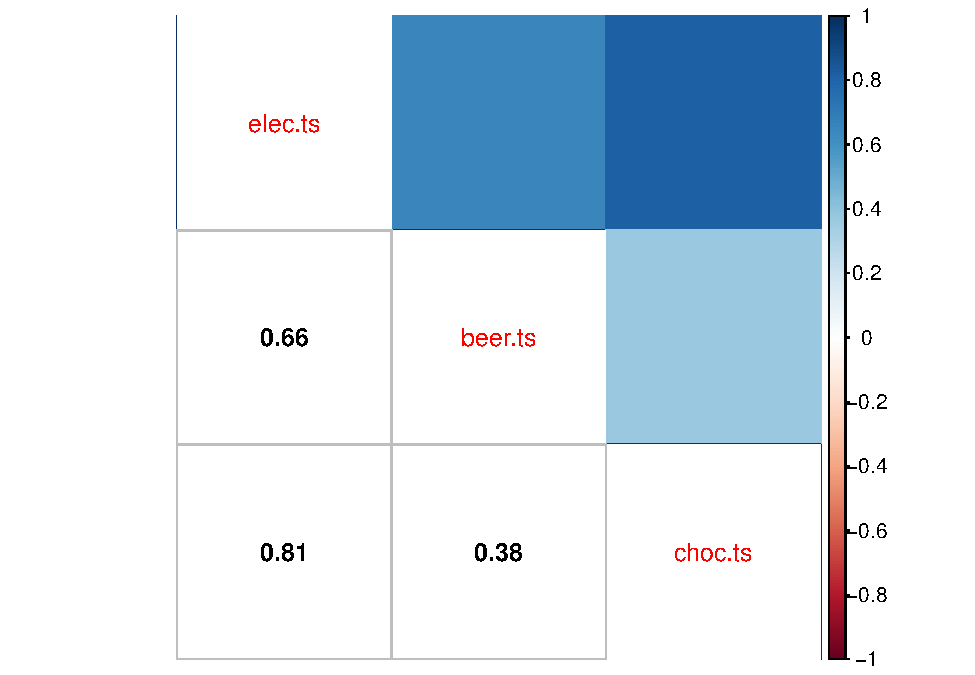
\includegraphics{TimeSeries_files/figure-latex/plotcorrelacion-1} 

}

\caption{Correlaciones sobre el consumo de electricidad y producción de cerveza y chocolate en Australia}\label{fig:plotcorrelacion}
\end{figure}

Para visualizar las tendencias de la serie se usará la función de \emph{aggregate()} para calcular las medias móviles y detectar gráficamente la tendencia sin el efecto de la periodicidad

\begin{Shaded}
\begin{Highlighting}[]
\NormalTok{cbe.tendencia }\OtherTok{=} \FunctionTok{aggregate}\NormalTok{(cbe.ts)}
\FunctionTok{plot}\NormalTok{(cbe.tendencia, }\AttributeTok{col=}\StringTok{\textquotesingle{}steelblue\textquotesingle{}}\NormalTok{, }
    \AttributeTok{main=}\StringTok{\textquotesingle{}Tendencia del consumo eléctrico\textquotesingle{}}\NormalTok{,}
    \AttributeTok{xlab=} \StringTok{\textquotesingle{}Tiempo\textquotesingle{}}\NormalTok{,}
    \AttributeTok{ylab=}\StringTok{\textquotesingle{}Miles de Wats/h\textquotesingle{}}\NormalTok{)}
\end{Highlighting}
\end{Shaded}

\begin{figure}

{\centering 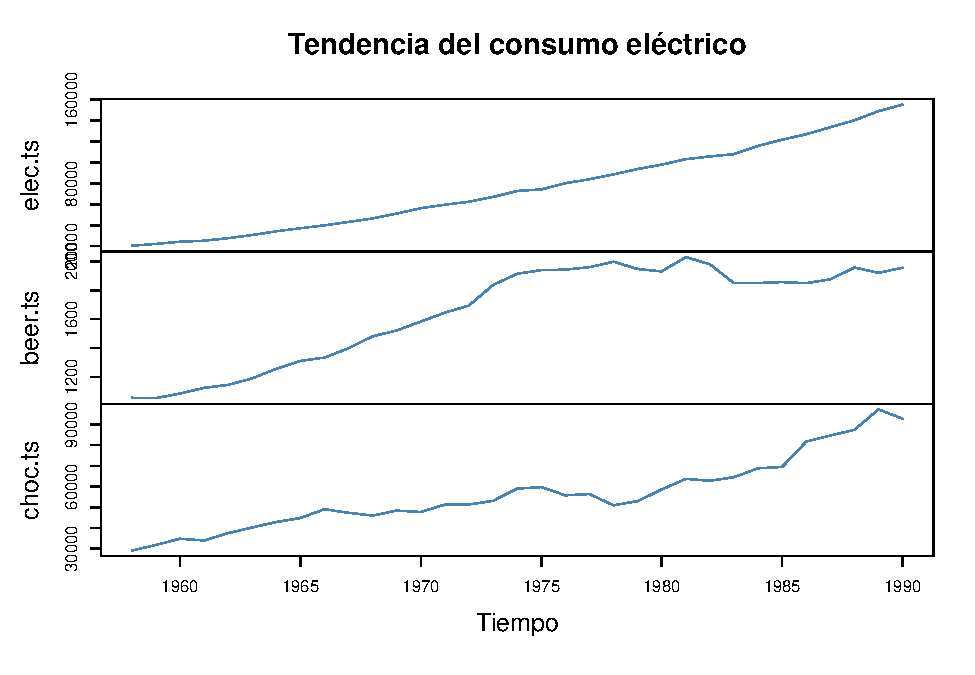
\includegraphics{TimeSeries_files/figure-latex/plottendenciamulti-1} 

}

\caption{Gráfica de las tendencias de la serie referentes a Australia}\label{fig:plottendenciamulti}
\end{figure}

Como se aprecia, el consumo de electricidad tiene una clara tendencia al alta, mientras que la producción de cerveza a pesar de que tenía un crecimiento constante de 1950 a 1974, desde 1975, la tendencia se mantiene constante con pequeñas subidas y bajadas en el tiempo. Por último, la producción de chocolate tiene una tendencia al alta, sin embargo, a lo largo del tiempo ha presentado incrementos y decrementos constantes en todo el intervalo de observación.

Para la ciclicidad, no existe una función que se pueda emplear sobre este objeto múltiple, así que se realizará la función \emph{ggseasonplot()} para consultar la variación estacional

\begin{Shaded}
\begin{Highlighting}[]
\FunctionTok{par}\NormalTok{(}\AttributeTok{mfrow=}\FunctionTok{c}\NormalTok{(}\DecValTok{1}\NormalTok{,}\DecValTok{3}\NormalTok{)) }\CommentTok{\#Permite graficar dos gráficas en una ventana}


\FunctionTok{ggseasonplot}\NormalTok{(elec.ts,}
             \AttributeTok{polar=}\ConstantTok{TRUE}\NormalTok{, }
             \AttributeTok{main=}\StringTok{"Periodicidad del consumo de energía eléctrica"}\NormalTok{ )}
\FunctionTok{ggseasonplot}\NormalTok{(beer.ts,}
             \AttributeTok{polar=}\ConstantTok{TRUE}\NormalTok{, }
             \AttributeTok{main=}\StringTok{"Periodicidad del consumo de la producción de cerveza"}\NormalTok{ )}
\FunctionTok{ggseasonplot}\NormalTok{(choc.ts,}
             \AttributeTok{polar=}\ConstantTok{TRUE}\NormalTok{, }
             \AttributeTok{main=}\StringTok{"Periodicidad del consumo de la producción de chocolate"}\NormalTok{ )}


\FunctionTok{par}\NormalTok{(}\AttributeTok{mfrow=}\FunctionTok{c}\NormalTok{(}\DecValTok{1}\NormalTok{,}\DecValTok{1}\NormalTok{))}
\end{Highlighting}
\end{Shaded}

\begin{figure}

{\centering 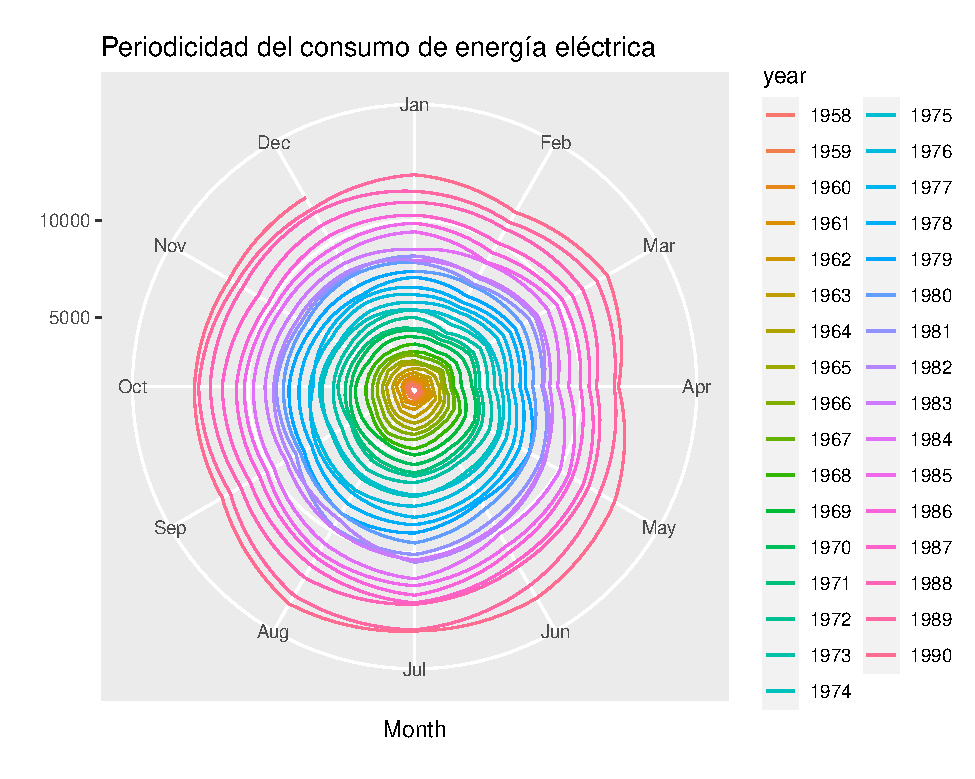
\includegraphics[width=0.33\linewidth]{TimeSeries_files/figure-latex/plotPeriodicidadcbe-1} 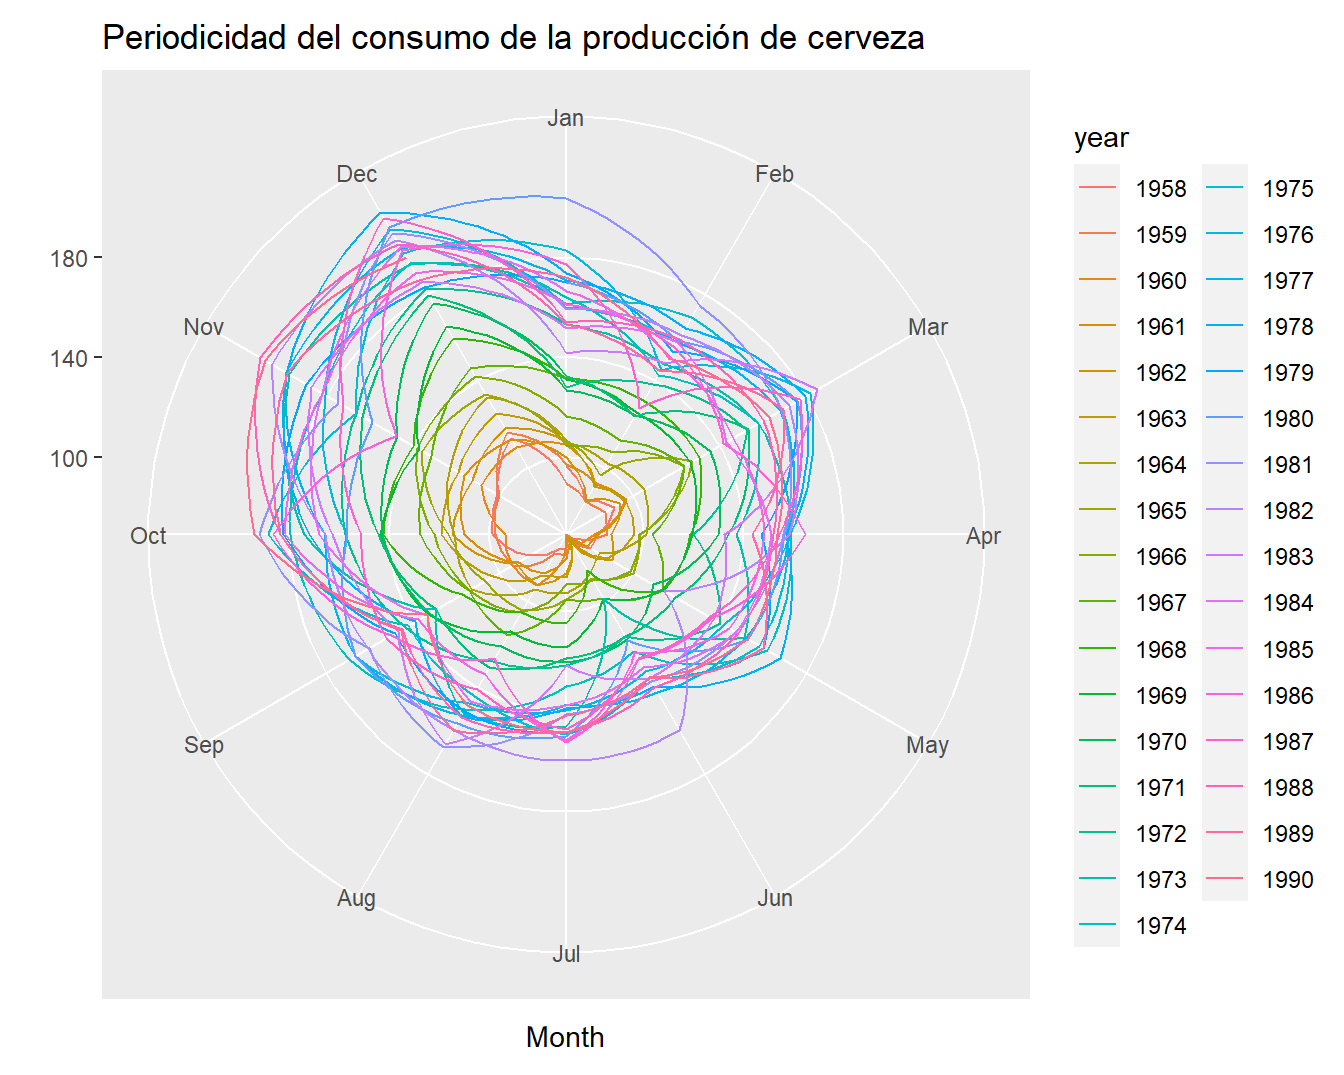
\includegraphics[width=0.33\linewidth]{TimeSeries_files/figure-latex/plotPeriodicidadcbe-2} 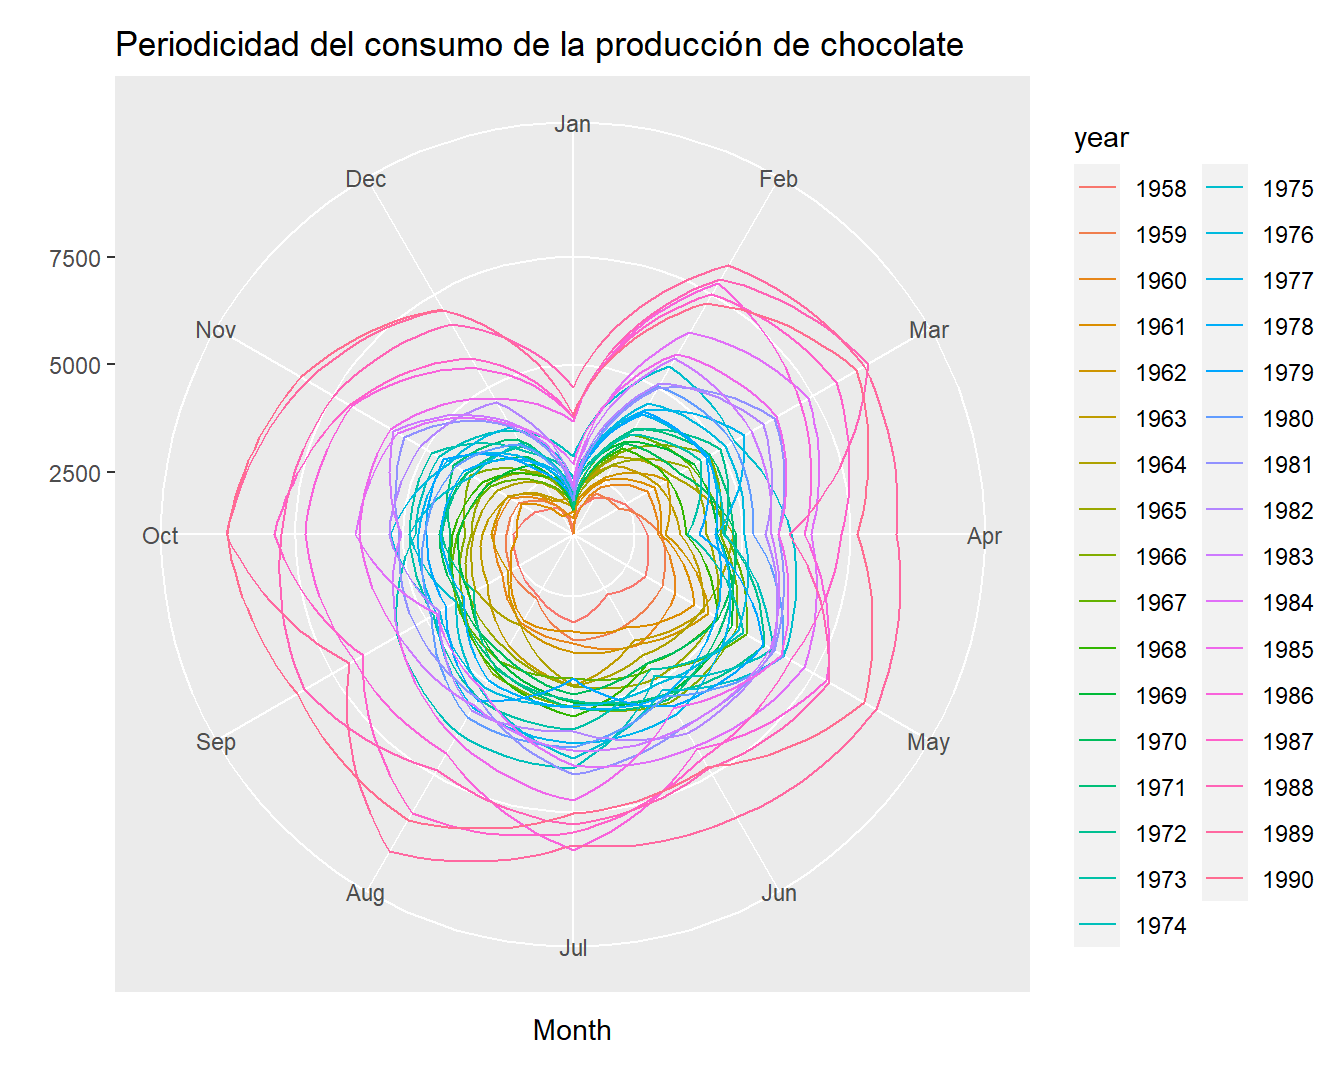
\includegraphics[width=0.33\linewidth]{TimeSeries_files/figure-latex/plotPeriodicidadcbe-3} 

}

\caption{Gráfica de la variación de la serie CBE}\label{fig:plotPeriodicidadcbe}
\end{figure}

Se decidió hacer la gráfica \ref{fig:plotPeriodicidadcbe} de manera polar, pues debido a la gran cantidad de años que se analizan el resultado no sería claramente visualizado. En dicha figura, se observa que la primera gráfica hace referencia a la variación estacional del consumo eléctrico, en ella se aprecia que el consumo se comporta de manera lineal a lo largo del año, aunque existe un mayor consumo en los meses de junio a agosto mientras que en abril hay un menor consumo. La segunda gráfica hace referencia a la producción de cerveza, el comportamiento es más variado año tras año, pero se puede apreciar que en enero y febrero sucede que la producción es muy baja, después empieza a aumentar paulatinamente hasta diciembre, mes en el cual se encuentra la mayor producción del año. Mientras que la producción de chocolate, la ciclicidad es fácil de observar, en enero la producción es muy baja posteriormente empieza a aumentar hasta agosto y octubre donde se realiza la mayor producción después de estas fechas la producción empieza a caer para el resto del año.

\hypertarget{pasajeros-auxe9reos}{%
\subsection{Pasajeros aéreos}\label{pasajeros-auxe9reos}}

Otra de la serie de tiempo que se estará analizando será \textbf{Air Passengers}, esta es posiblemente una de las series más utilizadas ya que se presenta a detalle en el texto Box \& Jenkins (1976) , uno de los libros pioneros en el análisis estadístico de las series de tiempo, aunque la recopilación de los datos y análisis corresponde a Brown (1962).

La base \textbf{Air Passengers} hace referencia al número de personas (en miles) que viajan mensualmente en una cierta aerolínea internacional de pasajeros durante el periodo de enero de 1949 a diciembre de 1960.

Debido a la gran importancia histórica y que es de gran utilidad para ilustrar los conceptos de la exploración de los datos de series de tiempo, esta base se encuentra precargada en R, sólo será necesario invocarla con el comando para poder utilizarla, \emph{AirPassengers}.

\begin{Shaded}
\begin{Highlighting}[]
\NormalTok{AP.ts }\OtherTok{=}\NormalTok{ AirPassengers}
\NormalTok{AP.ts}
\end{Highlighting}
\end{Shaded}

\begin{verbatim}
##      Jan Feb Mar Apr May Jun Jul Aug Sep Oct Nov Dec
## 1949 112 118 132 129 121 135 148 148 136 119 104 118
## 1950 115 126 141 135 125 149 170 170 158 133 114 140
## 1951 145 150 178 163 172 178 199 199 184 162 146 166
## 1952 171 180 193 181 183 218 230 242 209 191 172 194
## 1953 196 196 236 235 229 243 264 272 237 211 180 201
## 1954 204 188 235 227 234 264 302 293 259 229 203 229
## 1955 242 233 267 269 270 315 364 347 312 274 237 278
## 1956 284 277 317 313 318 374 413 405 355 306 271 306
## 1957 315 301 356 348 355 422 465 467 404 347 305 336
## 1958 340 318 362 348 363 435 491 505 404 359 310 337
## 1959 360 342 406 396 420 472 548 559 463 407 362 405
## 1960 417 391 419 461 472 535 622 606 508 461 390 432
\end{verbatim}

Como se aprecia, el resultado tiene un comportamiento parecido a un objeto \emph{ts} ya que la información se encuentra indexada y acomodado en el formato típico. Así que se comprobará esta suposición.

\begin{Shaded}
\begin{Highlighting}[]
\FunctionTok{class}\NormalTok{(AP.ts)}\CommentTok{\#El formato de la serie de tiempo es}
\end{Highlighting}
\end{Shaded}

\begin{verbatim}
## [1] "ts"
\end{verbatim}

\begin{Shaded}
\begin{Highlighting}[]
\FunctionTok{start}\NormalTok{(AP.ts)}\CommentTok{\#El incio de la serie de tiempo es}
\end{Highlighting}
\end{Shaded}

\begin{verbatim}
## [1] 1949    1
\end{verbatim}

\begin{Shaded}
\begin{Highlighting}[]
\FunctionTok{end}\NormalTok{(AP.ts)}\CommentTok{\#El fin de la serie de tiempo es}
\end{Highlighting}
\end{Shaded}

\begin{verbatim}
## [1] 1960   12
\end{verbatim}

\begin{Shaded}
\begin{Highlighting}[]
\FunctionTok{frequency}\NormalTok{(AP.ts)}\CommentTok{\#La frecuencia de la serie de tiempo es}
\end{Highlighting}
\end{Shaded}

\begin{verbatim}
## [1] 12
\end{verbatim}

\begin{Shaded}
\begin{Highlighting}[]
\FunctionTok{summary}\NormalTok{(AP.ts) }\CommentTok{\#Información de la distribución de los datos}
\end{Highlighting}
\end{Shaded}

\begin{verbatim}
##    Min. 1st Qu.  Median    Mean 3rd Qu.    Max. 
##   104.0   180.0   265.5   280.3   360.5   622.0
\end{verbatim}

Debido a la función \emph{class()} se conoce que efectivamente \emph{AirPassengers} al ser una base precargada tiene este procesamiento por lo que no es necesario volver a definir los datos como objeto \emph{ts}. De igual manera se observa que los datos tienen una periodicidad mensual en el cual el primer dato es registrado en enero de 1949 y el último en diciembre de 1960. El valor de miles de personas que viajan en esa Aerolínea es 104, las personas medias 265.5 y el valor máximo que se tuvo registro fue 622 mil pasajeros interesados en viajar con esta aerolínea.

Ya que los datos se encuentran previamente creados, sólo se realizarán las gráficas basadas en \emph{ts} y el objeto \emph{xts} los cuales puedes consultarse en la gráfica \ref{fig:plotAP}, al estar ya creado este objeto facilita mucho el análisis y la generación de los diagramas mostrados.

\begin{Shaded}
\begin{Highlighting}[]
\FunctionTok{par}\NormalTok{(}\AttributeTok{mfrow=}\FunctionTok{c}\NormalTok{(}\DecValTok{2}\NormalTok{,}\DecValTok{1}\NormalTok{))}

\FunctionTok{plot}\NormalTok{(AP.ts,  }\AttributeTok{xlab=} \StringTok{\textquotesingle{}Tiempo\textquotesingle{}}\NormalTok{, }
     \AttributeTok{ylab =} \StringTok{\textquotesingle{}Miles de pasajeros\textquotesingle{}}\NormalTok{,}
     \AttributeTok{main =} \StringTok{\textquotesingle{}Frecuencia de pasajeros de una aerolínea\textquotesingle{}}\NormalTok{,}
     \AttributeTok{col=}\StringTok{\textquotesingle{}steelblue\textquotesingle{}}\NormalTok{)}

\NormalTok{AP.xts }\OtherTok{=} \FunctionTok{as.xts}\NormalTok{(AP.ts)}
\FunctionTok{plot}\NormalTok{(AP.xts,}
      \AttributeTok{xlab=} \StringTok{\textquotesingle{}Tiempo\textquotesingle{}}\NormalTok{, }
     \AttributeTok{ylab =} \StringTok{\textquotesingle{}Miles de pasajeros\textquotesingle{}}\NormalTok{,}
      \AttributeTok{col =} \StringTok{\textquotesingle{}steelblue\textquotesingle{}}\NormalTok{, }
     \AttributeTok{grid.ticks.on =} \StringTok{\textquotesingle{}quarters\textquotesingle{}}\NormalTok{, }\CommentTok{\#Crea líneas verticales sobre la gráfica cada trimestre}
     \AttributeTok{major.ticks =} \StringTok{\textquotesingle{}quarters\textquotesingle{}}\NormalTok{,  }\CommentTok{\#Crea líneas verticales sobre la gráfica cada trimestre}
     \AttributeTok{minor.ticks =}\StringTok{\textquotesingle{}years\textquotesingle{}}\NormalTok{, }\CommentTok{\# Escribe la etiqueta de los meses cada cierto tiempo}
     \AttributeTok{grid.col =} \StringTok{\textquotesingle{}lightgrey\textquotesingle{}}\NormalTok{, }\CommentTok{\#color líneas verticales}
     \AttributeTok{main=}\StringTok{\textquotesingle{}Frecuencia de pasajeros de una aerolínea\textquotesingle{}}
     
\NormalTok{     )}



\FunctionTok{par}\NormalTok{(}\AttributeTok{mfrow=}\FunctionTok{c}\NormalTok{(}\DecValTok{1}\NormalTok{,}\DecValTok{1}\NormalTok{))}
\end{Highlighting}
\end{Shaded}

\begin{figure}

{\centering 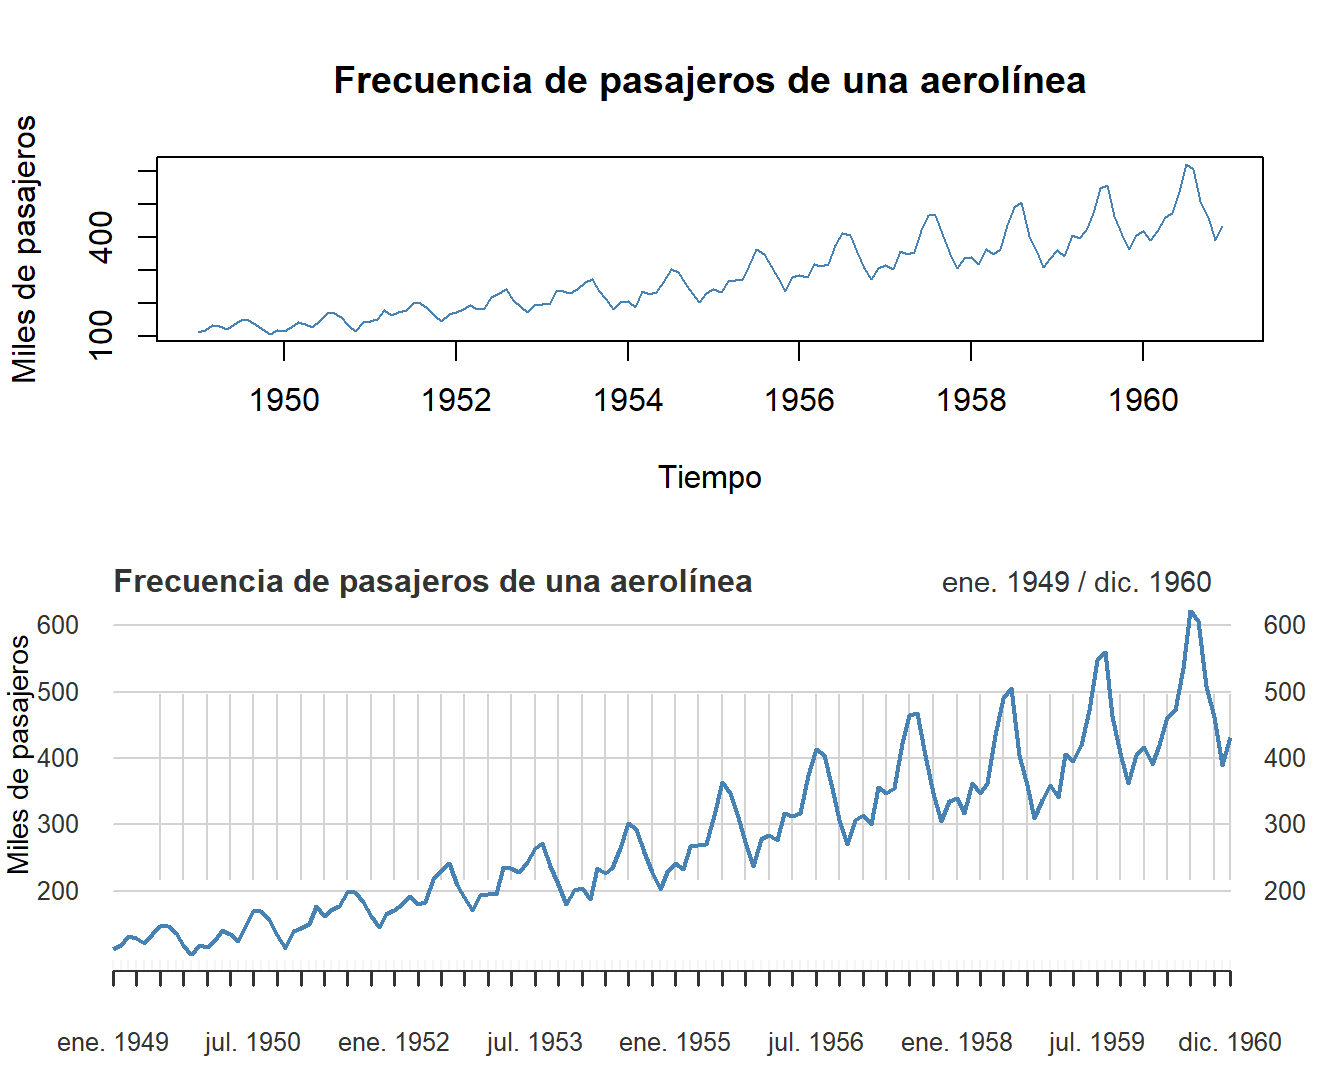
\includegraphics[width=1\linewidth]{TimeSeries_files/figure-latex/plotAP-1} 

}

\caption{Gráfica de frecuencia de pasajeros de una aerolínea.}\label{fig:plotAP}
\end{figure}

En la gráfica \ref{fig:plotAP} se puede notar que la gráfica superior corresponde a la representación por medio del objeto \emph{ts}, mientras que la inferior al objeto \emph{xts}. Ambas gráficas muestran la misma información, sin embargo, debido a la construcción del \emph{xts} permite un mayor control y ubicación en el tiempo pues presenta líneas auxiliares dentro de la misma gráfica.

De manera general se puede concluir que la cantidad de pasajeros de esta aerolínea tiene una tendencia positiva pues conforme pasa el tiempo una mayor cantidad de personas están realizando un viaje en esta aerolínea, de igual manera, existe un ciclo o periodicidad anual en el cual cada año se puede percibir una clara variación estacional en el cual a inicios de año la cantidad de vuelos es menor pero aumentando paulatinamente hasta la temporada vacacional de verano donde se alcanzan los máximos por año y de ahí empieza a disminuir para el resto del año. Se aprecia que conforme aumenta el tiempo más variabilidad existen en los datos, pues al comienzo la varianza de los datos visualmente es menor y en tiempos posteriores la varianza aumenta creando ciclos cada vez más pronunciados. Estos comentarios son respaldados con las gráficas contenidas en la figura \ref{fig:clipeAP}.

\begin{Shaded}
\begin{Highlighting}[]
\FunctionTok{par}\NormalTok{(}\AttributeTok{mfrow=}\FunctionTok{c}\NormalTok{(}\DecValTok{2}\NormalTok{,}\DecValTok{1}\NormalTok{))}
\DocumentationTok{\#\# Tendencia}
\NormalTok{AP.tendencia }\OtherTok{=} \FunctionTok{aggregate}\NormalTok{(AP.ts)}

\FunctionTok{plot}\NormalTok{(AP.tendencia, }\AttributeTok{col=}\StringTok{\textquotesingle{}steelblue\textquotesingle{}}\NormalTok{, }
    \AttributeTok{main=}\StringTok{\textquotesingle{}Tendencia de la cantidad de pasajeros\textquotesingle{}}\NormalTok{,}
    \AttributeTok{xlab=} \StringTok{\textquotesingle{}Tiempo\textquotesingle{}}\NormalTok{,}
    \AttributeTok{ylab=}\StringTok{\textquotesingle{}Miles pasajeros\textquotesingle{}}\NormalTok{)}

\CommentTok{\# Periodicidad}
\FunctionTok{boxplot}\NormalTok{(AP.ts }\SpecialCharTok{\textasciitilde{}} \FunctionTok{cycle}\NormalTok{(AP.ts),}
        \AttributeTok{col =} \StringTok{"orange"}\NormalTok{, }\CommentTok{\# Color de relleno}
        \AttributeTok{border =} \StringTok{"brown"}\NormalTok{, }\CommentTok{\#Color de contorno}
        \AttributeTok{main=}\StringTok{\textquotesingle{}Peridicidad de la cantidad de pasajeros\textquotesingle{}}\NormalTok{,}
        \AttributeTok{xlab=} \StringTok{\textquotesingle{}Tiempo\textquotesingle{}}\NormalTok{,}
        \AttributeTok{ylab=}\StringTok{\textquotesingle{}Miles pasajeros\textquotesingle{}}\NormalTok{,}
        \AttributeTok{names =}\NormalTok{ month.abb }\CommentTok{\# Agregar nombres puede ser month.abb o month.name o }
                          \CommentTok{\#cualquier vector personalizado}
\NormalTok{        )}

\FunctionTok{par}\NormalTok{(}\AttributeTok{mfrow=}\FunctionTok{c}\NormalTok{(}\DecValTok{1}\NormalTok{,}\DecValTok{1}\NormalTok{))}
\end{Highlighting}
\end{Shaded}

\begin{figure}

{\centering 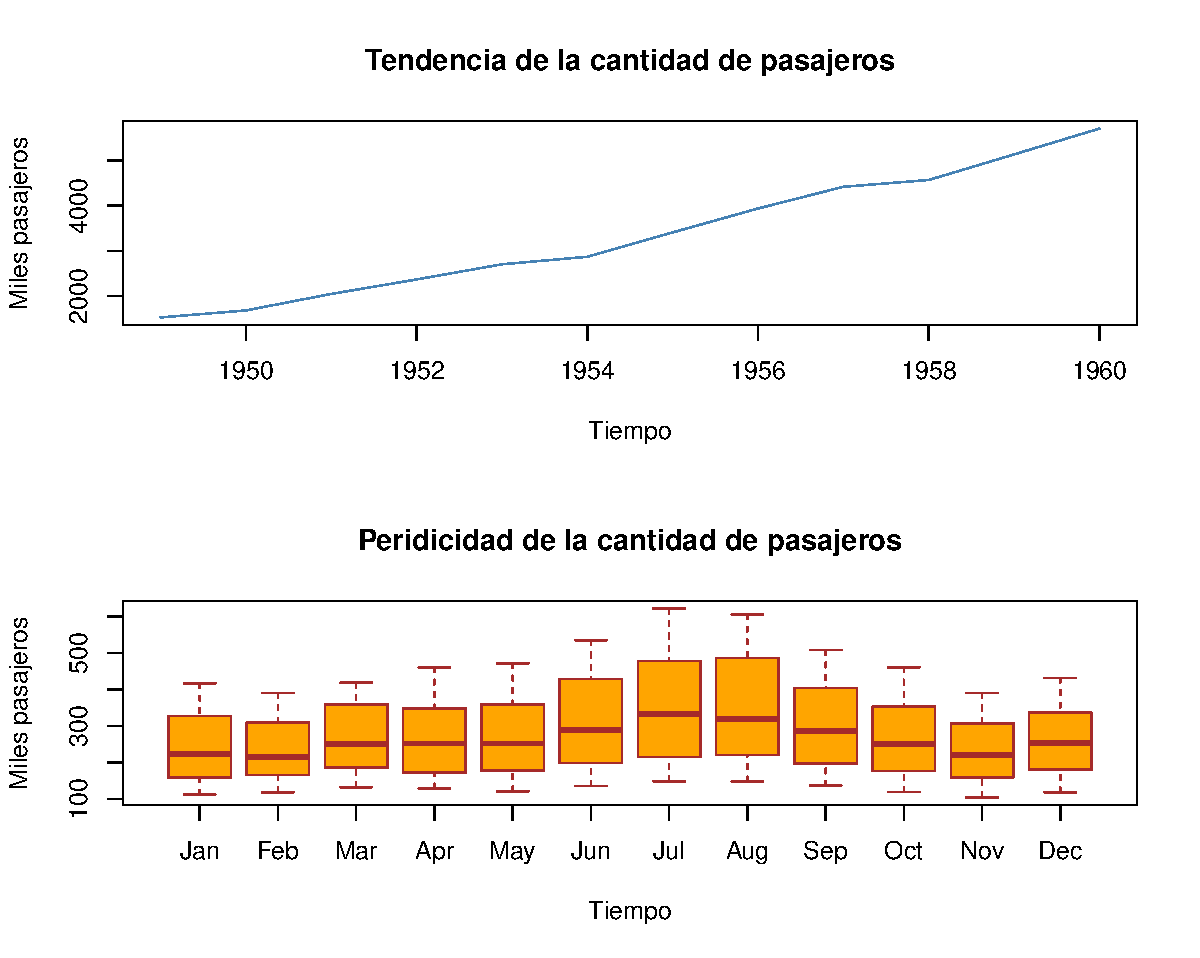
\includegraphics[width=1\linewidth]{TimeSeries_files/figure-latex/clipeAP-1} 

}

\caption{Periodicidad y tendencia de pasajeros de una aerolínea.}\label{fig:clipeAP}
\end{figure}

Como se aprecia en la figura \ref{fig:clipeAP} se refuerzan los comentarios anteriores, existe un aumento progresivo a lo largo del tiempo de manera creciente lineal por lo que se dice que sigue una tendencia. Se observa una periodicidad en forma de campana en el cual la mayor cantidad de viajes ocurre en julio y agosto, después de estas fechas existe un decrecimiento en la cantidad de vuelos.
Es importante tratar de describir el motivo de estos cambios, pues de esta manera, las estimaciones y resultados pueden evaluarse para decidir si se apegan o no a los datos. Así el aumento de la demanda de viajes aéreos puede debido a precios más competitivos, mayor disponibilidad de aviones o la apertura comercial que se ha vivido en últimas fechas, así como tratados internacionales han permitido que acceder a otros países sea más sencillo y las personas se encuentren más motivados a realizar estos viajes; la demanda en determinadas épocas del año corresponde a los periodos vacacionales, lo que podría explicar la variación estacional. Por otra parte, el aumento de la población podría explicar la tendencia al aumento constante.

  \bibliography{book.bib,packages.bib}

\end{document}
